%!/usr/bin/pdflatex

% The French Pratham ground station software system
%
% Author : Hai Nguyen Van,
% Institut de Physique du Globe de Paris, Université Paris Diderot
%
% The copyright to this code is held by Institut de Physique du Globe de Paris. All rights reserved. This file is distributed under the license CeCILL Free Software License Agreement.


% Use the following line for draft mode (double spaced, single column)
%\documentclass[preprint,pre,floats,aps,amsmath,amssymb]{revtex4}

% Use the following line for journal mode (single spaced, double column)
\documentclass[twocolumn,pre,floats,aps,amsmath,amssymb]{revtex4}
\usepackage{graphicx}
\usepackage{bm}
\usepackage{color}
\usepackage{multirow}
\usepackage{version}
\usepackage{hyperref}
\usepackage{algorithm}
\usepackage{algorithmic}
\usepackage{amssymb}
\usepackage{amsmath}
\usepackage{marvosym}
\usepackage{rotating}
%\usepackage[final]{pdfpages}
\usepackage{tikz}
\usetikzlibrary{automata,positioning}

%%% francisation des algorithmes
\renewcommand{\algorithmicrequire} {\textbf{\textsc{Entr\'ees:}}}
\renewcommand{\algorithmicensure}  {\textbf{\textsc{Sorties:}}}
\renewcommand{\algorithmicwhile}   {\textbf{tantque}}
\renewcommand{\algorithmicdo}      {\textbf{faire}}
\renewcommand{\algorithmicendwhile}{\textbf{fin tantque}}
\renewcommand{\algorithmicend}     {\textbf{fin}}
\renewcommand{\algorithmicif}      {\textbf{si}}
\renewcommand{\algorithmicendif}   {\textbf{finsi}}
\renewcommand{\algorithmicelse}    {\textbf{sinon}}
\renewcommand{\algorithmicthen}    {\textbf{alors}}
\renewcommand{\algorithmicfor}     {\textbf{pour}}
\renewcommand{\algorithmicforall}  {\textbf{pour tout}}
\renewcommand{\algorithmicdo}      {\textbf{faire}}
\renewcommand{\algorithmicendfor}  {\textbf{fin pour}}
\renewcommand{\algorithmicloop}    {\textbf{boucler}}
\renewcommand{\algorithmicendloop} {\textbf{fin boucle}}
\renewcommand{\algorithmicrepeat}  {\textbf{r\'ep\'eter}}
\renewcommand{\algorithmicuntil}   {\textbf{jusqu'\`a}}
\renewcommand{\algorithmicreturn}   {\textbf{retourner}}

\floatname{algorithm}{Algorithme}

%%%%%%%%%%%%%%%%%%%%%%%%%%%%%%%%%%%%%%%%%%%%%%%%%%%%%%%%%%%%%%%%%%%%%%%%%%%%%
\newtheorem{theorem}{Th\'eor\`eme.}[section]
\newtheorem{lemma}[theorem]{Lemme.}
\newtheorem{proposition}[theorem]{Proposition.}
\newtheorem{corollary}[theorem]{Corollaire.}
%\newtheorem{algorithm}[theorem]{Algorithme.}

\newenvironment{implementation}[1][Impl\'ementation.]{\begin{trivlist}
\item[\hskip \labelsep {\bfseries #1}]}{\end{trivlist}}

\newenvironment{proof}[1][D\'emonstration.]{\begin{trivlist}
\item[\hskip \labelsep {\bfseries #1}]}{\end{trivlist}}

\newenvironment{notation}[1][Notation.]{\begin{trivlist}
\item[\hskip \labelsep {\bfseries #1}]}{\end{trivlist}}


\newenvironment{definition}[1][D\'efinition.]{\begin{trivlist}
\item[\hskip \labelsep {\bfseries #1}]}{\end{trivlist}}
\newenvironment{example}[1][Exemple.]{\begin{trivlist}
\item[\hskip \labelsep {\bfseries #1}]}{\end{trivlist}}
\newenvironment{remark}[1][Remarque.]{\begin{trivlist}
\item[\hskip \labelsep {\bfseries #1}]}{\end{trivlist}}
%%%%%%%%%%%%%%%%%%%%%%%%%%%%%%%%%%%%%%%%%%%%%%%%%%%%%%%%%%%%%%%%%%%%%%%%%%%%%

\definecolor{rltgreen}{rgb}{0,0.5,0}
\definecolor{rltred}{rgb}{0.75,0,0}
\definecolor{grey}{rgb}{0.75,0.75,0.75}
\definecolor{oneblue}{rgb}{0,0,0.75}

\begin{document}

\title{The French Pratham ground station software system}
\author{\'Equipe Pratham}
\affiliation{Universit\'e Paris Diderot $-$ Institut de Physique du Globe de Paris, 4 avenue de Neptune, 94100 Saint-Maur-des-Foss\'es, France}
\date{\today}

\begin{abstract}
  The copyright to this document and its source code are held by Institut de Physique du Globe de Paris. All rights reserved. This file is distributed under the license CeCILL Free Software License Agreement~\cite{cecill}.
\end{abstract}

\maketitle

\section{Introduction}
\label{sec:intro}

The following application note introduces technical issues related to the control-data-acquistion software system of the ground station at IPGP for Pratham satellite~\cite{IITB_general}. It aims to give scientific answers to the choice of implemented structures, including: antenna rotor control, time-based acquisition scheduler, \textsc{fsk} (\textsc{frequency-shift keying}) and \textsc{ook} (\textsc{on-off keying}) demodulation, \textsc{ax.25} frame decoding, \textsc{morse} code decoding and data recording.

\textbf{Warning.} Section marks { \color{rltred}{\Radioactivity} } give scientific arguments but not necessarily relevant information for the understanding of this document. Some algorithm implementation details have been omitted for more abstraction towards specific programming languages.

\subsection{Sch\'ema d'acquisition g\'en\'eral}

The \texttt{NI-6353}~\cite{NI_6353_datasheet}~\cite{NI_calibration_procedure} Acquisition Box (considered as an ADC) acquires twelve voltage measurements in volt (V).

\begin{table}[ht]
  \caption{Set of voltage measurements to acquire}
  \begin{center}
    \begin{footnotesize}
      \begin{tabular}{|c|c|c|rcc|}
        \hline
        \multirow{7}{*}{145,980 MHz antenna} & \multirow{3}{*}{Plane 1} & \multirow{3}{*}{$\dots$} & VR5000          & \color{rltgreen}{$\rightarrow$} & \multirow{14}{*}{NI-6353}\\ \cline{4-5}
        &                         &                          & AD8302$_{mag}$   & \color{oneblue}{$\rightarrow$} & \\ \cline{4-5}
        &                         &                          & AD8302$_{phase}$ & \color{oneblue}{$\rightarrow$} & \\ \cline{2-5}
        & \multirow{3}{*}{Plane 2} & \multirow{3}{*}{$\dots$} & VR5000          & \color{rltgreen}{$\rightarrow$} & \\ \cline{4-5}
        &                         &                          & AD8302$_{mag}$   & \color{oneblue}{$\rightarrow$} & \\ \cline{4-5}
        &                         &                          & AD8302$_{phase}$ & \color{oneblue}{$\rightarrow$} & \\ \cline{1-5}
        
        \multirow{7}{*}{437,455 MHz antenna} & \multirow{3}{*}{Plane 1} & \multirow{3}{*}{$\dots$} & VR5000          & \color{rltred}{$\rightarrow$}  & \\ \cline{4-5}
        &                         &                          & AD8302$_{mag}$   & \color{oneblue}{$\rightarrow$} & \\ \cline{4-5}
        &                         &                          & AD8302$_{phase}$ & \color{oneblue}{$\rightarrow$} & \\ \cline{2-5}
        & \multirow{3}{*}{Plane 2} & \multirow{3}{*}{$\dots$} & VR5000          & \color{rltred}{$\rightarrow$} & \\ \cline{4-5}
        &                         &                          & AD8302$_{mag}$   & \color{oneblue}{$\rightarrow$} & \\ \cline{4-5}
        &                         &                          & AD8302$_{phase}$ & \color{oneblue}{$\rightarrow$} & \\ \cline{4-5}
        
        \hline
      \end{tabular}
    \end{footnotesize}
  \end{center}
  \label{tab:diagramme_gen}
\end{table}

\begin{remark}
  We introduce on \textsc{table}~\ref{tab:diagramme_gen} a flowchart of acquisition channels at the input of ADC. { \color{oneblue}{Blue} } arrows ($\rightarrow$) match with channels from which the ADC acquire voltage measurements (in Volts). In the same way, { \color{rltgreen}{green} } (resp. { \color{rltred}{red} }) arrows match with as well voltage measurements acquisition as \textsc{ook} demodulation and \textsc{Morse} decoding (resp. \textsc{fsk} demodulation and \textsc{ax.25} frame decoding).
\end{remark}

\subsection{Digital signal at 437,455 MHz : Health monitoring data}

The following process is applied to the two channels specified by { \color{rltred}{red} } arrows of the previous flowchart. At the end of the process we then have two output files for the same information $-$ as a matter of fact $-$ more accuracy.

\begin{figure}[h]
  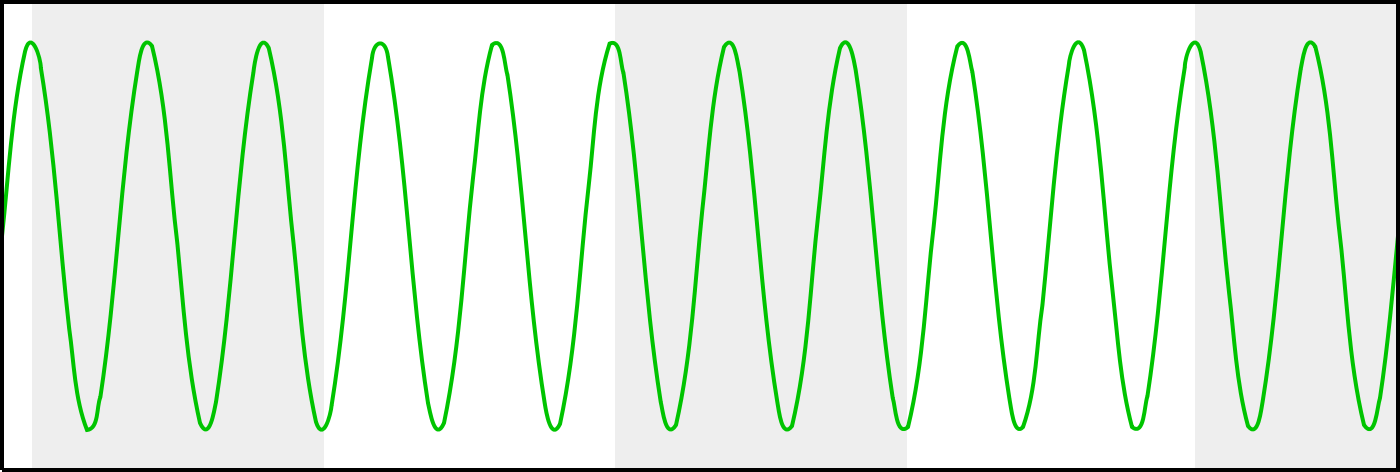
\includegraphics[width=8cm]{pictures/porteuse.png}
  \caption{Carrier signal (central frequency $F_c$)}
  \label{fig:signal_porteur}
\end{figure}

\begin{figure}[h]
  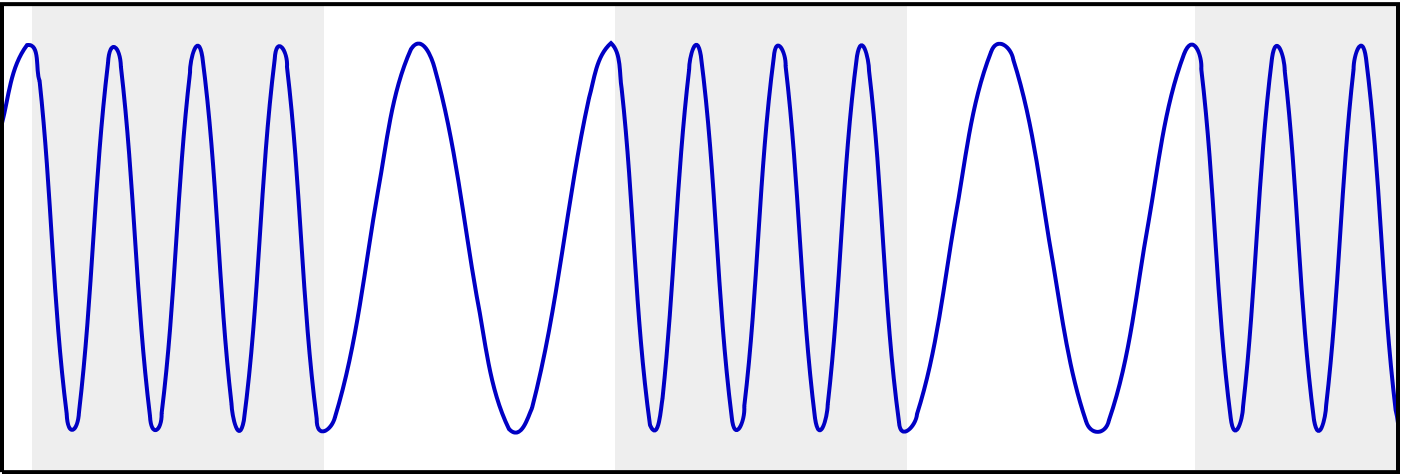
\includegraphics[width=8cm]{pictures/signal_mod.png}
  \caption{Modulated signal in \textsc{fsk} at $F_c \pm \frac{\Delta f}{2}$ frequencies received by the \texttt{VR5000}}
  \label{fig:signal_module}
\end{figure}

\begin{figure}[h]
  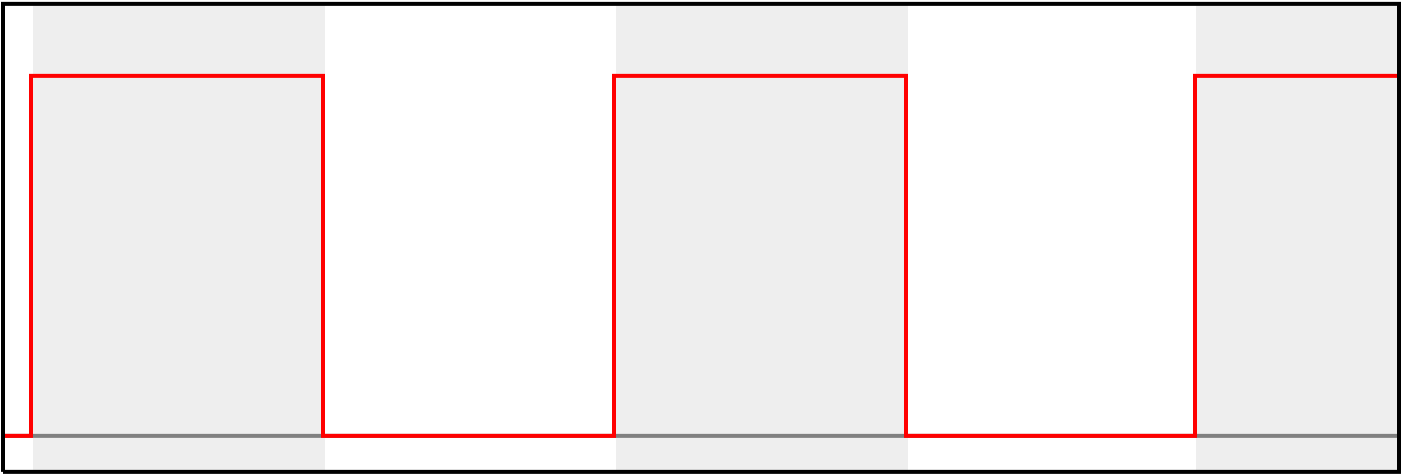
\includegraphics[width=8cm]{pictures/signal_demod.png}
  \caption{Modulating signal at $F_b = 1,2 \ \operatorname{kbit}.\operatorname{s}^{-1}$ bit rate (retrieved by \textsc{fsk} demodulation)}
  \label{fig:signal_modulant}
\end{figure}

The satellite sends a signal with a declared carrier signal at $F_c = 437,455$ MHz (\textsc{figure}~\ref{fig:signal_porteur}) and a passband bandwidth of $\Delta f = 9,90$ kHz (ref ?). At the end of the acquisition chain the \textsc{vr5000} transceiver acquires a signal whose central frequency is $F_c$ and whose passband bandwidth is $\Delta f$ (\textsc{figure}~\ref{fig:signal_module}).

The transceiver returns an audio signal. It finally decribes $-$ through a Schmitt trigger (ref ?) $-$ the modulating signal (\textsc{figure}~\ref{fig:signal_modulant}). The digital baseband transmission method is of the kind non-return-to-zero (\textsc{nrz})~\cite{nrz_gorry} (ref ?). The data bits are then saved in a file in such a way that (more info on peak sync ? method not sure...)

La d\'emodulation effectu\'ee par le transceiver renvoie un signal audio, correspondant directement au \textit{signal modulant} (\textsc{figure}~\ref{fig:signal_modulant}). Les changements d'\'etats codent les bits de donn\'ees en NRZ~\cite{nrz_gorry}. Ces bits de donn\'ees sont par la suite enregistr\'es dans un fichier de telle fa\c{c}on que $-$ sur une p\'eriode $T_b$ $-$ la pr\'esence d'une amplitude positive non-n\'egligeable (moyenne du signal sur une dur\'ee $T_b$) corresponde au \texttt{1} logique et son l'amplitude nulle au \texttt{0}. Ces bits de donn\'ees sont par la suite enregistr\'es dans un fichier (\textsc{figure}~\ref{fig:bits_donnees}).

%On termine la d\'emodulation \texttt{FSK} en calculant, par \textit{transform\'ee de Fourier}, les amplitudes associ\'ees aux composantes fr\'equentielles $0$ et $1,2$ kHz sur une largeur de fen\^etre de calcul $\Delta t = \frac{1}{F_b}$.

\begin{figure}[h]
  \begin{tabular}{|c|}
    \hline
    $\dots$
    \textcolor{rltred}{$\underbrace{\texttt{01111110}}_{\textup{debut de trame}}$}
    $\dots$
    \textcolor{rltgreen}{$\underbrace{\texttt{10101010}}_{\textup{information}}$}
    $\dots$
    \textcolor{rltred}{$\underbrace{\texttt{01111110}}_{\textup{fin de trame}}$}
    $\dots$\\
    \hline
  \end{tabular}
\caption{Bits de donn\'ees correspondant au signal modulant}
\label{fig:bits_donnees}
\end{figure}

On ne s'int\'eresse cependant qu'\`a une partie des bits de donn\'ees. L'information issue du satellite $-$ cod\'ee en \texttt{AX.25} $-$ assure une fiabilit\'e dans la transmission de l'information. On d\'ecoupe alors les bits en donn\'ees en trames (\textsc{figure}~\ref{fig:bits_sans_ax25}).

\begin{figure}[h]
  \begin{tabular}{|c|}
    \hline
    $\dots$ \textcolor{rltgreen}{\texttt{10101010}} $\dots$\\
    \hline
  \end{tabular}
  \caption{Bits de donn\'ees d\'ecod\'ees des trames \texttt{AX.25}}
  \label{fig:bits_sans_ax25}
\end{figure}

Les bits restants du d\'ecoupage sont alors les bits de donn\'ees au format d\'efinies par l'\textsc{iitb}\cite{IITB}.

\subsection{Signal num\'erique \`a 145,980 MHz : Beacon}

De mani\`ere analogue, le transceiver d\'emodule un signal \`a fr\'equence centrale $F_c = 145,980$ MHz (\textsc{figure}~\ref{fig:signal_ook}). Avec un d\'ebit binaire de $F_b = 10 \ \operatorname{bit}.\operatorname{s}^{-1}$, la pr\'esence de la composante fr\'equentielle $F_c$ indique une impulsion et, celle de la composante $0$, aucune impulsion (On-Off Keying) (\textsc{figure}~\ref{fig:impulsions_morse}).

\begin{figure}[h]
  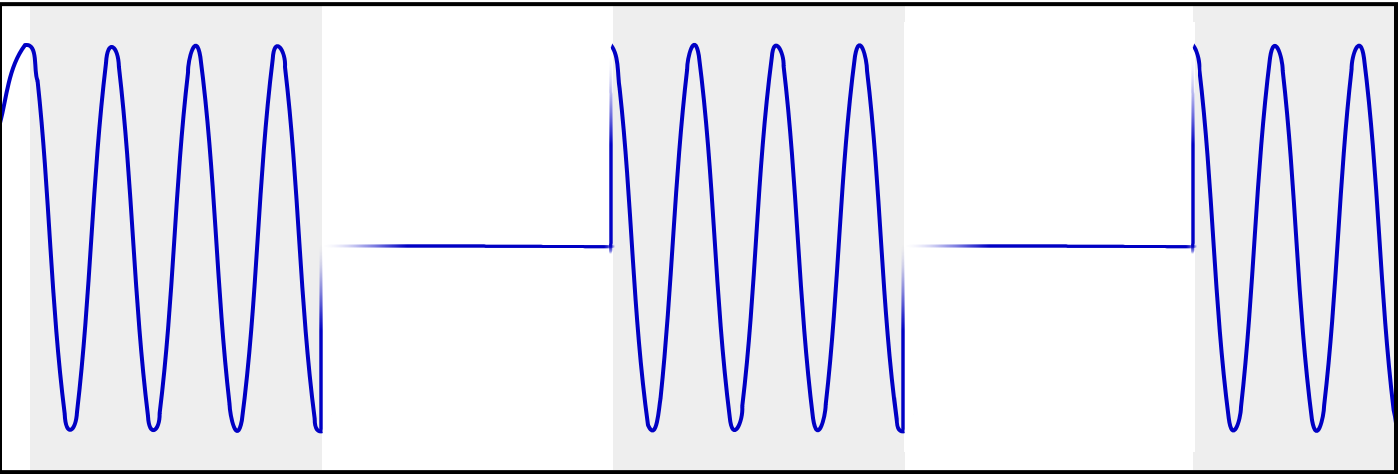
\includegraphics[width=8cm]{pictures/sans_porteuse.png}
  \caption{Signal modul\'e en \texttt{OOK} \`a fr\'equence $F_c$ re\c{c}u par le \texttt{VR5000}}
  \label{fig:signal_ook}
\end{figure}

On d\'echiffre ensuite l'information cod\'ee en morse suivant la longueur des impulsions (trait long ou trait court) suivant le syst\`eme de codage international (\textsc{figure}~\ref{fig:info_decode_morse}).

\begin{figure}[]
  \begin{tabular}{|c|}
    \hline
    $\dots$ \textcolor{rltred}{\texttt{...- ..- ..--- -- -.. --.-}} $\dots$\\
    \hline
  \end{tabular}
  \caption{Signal num\'eris\'e correspondant \`a des impulsions}
  \label{fig:impulsions_morse}
\end{figure}

\begin{figure}[]
  \begin{tabular}{|c|}
    \hline
    $\dots$ \textcolor{rltgreen}{\texttt{VU2MDQ}} $\dots$\\
    \hline
  \end{tabular}
  \caption{Information d\'ecod\'ee du code morse}
  \label{fig:info_decode_morse}
\end{figure}

On applique alors un tel traitement aux deux voies (fl\`eches { \color{rltgreen}{vertes} } sur le sch\'ema pr\'ec\'edent) afin d'obtenir deux informations et donc plus de pr\'cision.

\subsection{Rapports de gain et de phase : information sur le TEC}

Huit voies (fl\`eches { \color{oneblue}{bleues} } du sch\'ema pr\'ec\'edent) sont d\'edi\'es \`a l'acquisition de rapports de gain et de phase, issus des \texttt{AD8302}. On enregistre directement en fichier les mesures de tensions des huit voies restantes. Un post-traitement de ces valeurs sera effectu\'e avec Matlab afin de r\'ecup\'erer l'information sur le \textsc{tec}.

\section{Th\'eories et impl\'ementations}
\label{sec:theory}

\subsection{Contr\^ole motoris\'e de l'antenne}

\begin{figure}[h]
  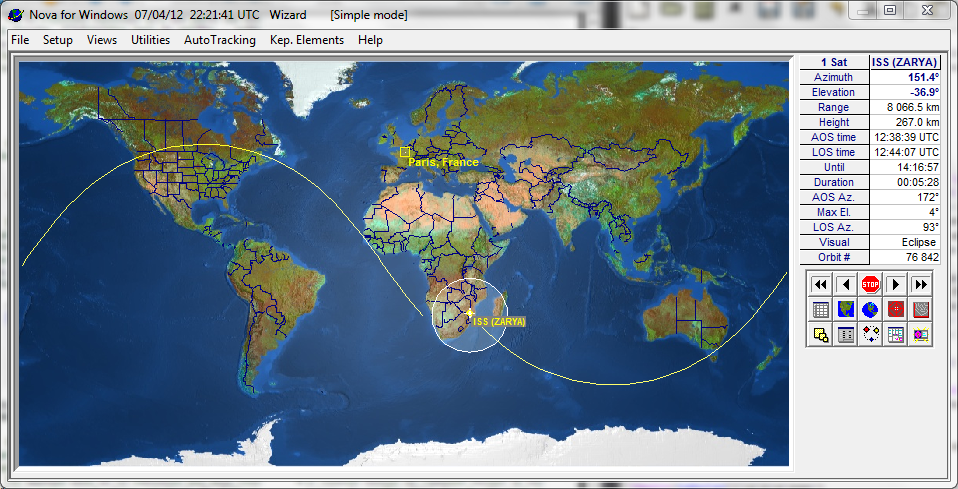
\includegraphics[width=8cm]{pictures/nova3.png}
\caption{Logiciel \texttt{Nova} de NLSA}
\label{fig:geometry}
\end{figure}

Le contr\^ole de la position des axes de l'antenne est enti\`erement g\'er\'ee par le logiciel \texttt{NLSA Nova}~\cite{nova_um}. Le contr\^oleur de l'antenne \'etant reli\'e \`a l'ordinateur par \texttt{RS-232}, Nova g\`ere \`a la fois :
\begin{itemize}
\item{la gestion et la mise \`a jour de la base de donn\'ees sur les positions des satellites (\href{https://www.space-track.org}{Space-Track});}
\item{la g\'en\'eration d'informations sur les e\'le\'vations minimales et maximales de satellites ;}
\item{le contr\^ole moteur de l'antenne suivant la trajectoire du satellite d\'esir\'e dans le r\'ef\'erentiel de l'antenne.}
\end{itemize}

\begin{remark}
  Pour les d\'etails techniques sur la mise en route de \texttt{Nova}, cf. \textsc{Appendix II}.
\end{remark}

\subsection{Gestion du temps et minuterie}

\textbf{Technique.} Les donn\'ees de temps n\'ecessaires \`a la mise en route de la minuterie sont fournies par \texttt{Nova} (fichier \texttt{Nova listing data.TXT}) en suivant la proc\'edure suivante :
\begin{enumerate}
\item {Choisir le satellite et le r\'ef\'erentiel de pr\'ef\'erence (\texttt{Configure current view})}
\item {\textup{Utilities} $\rightarrow$ \textup{Listing}}
\item {\textup{One Observer AOS/LOS} $\rightarrow$ \textup{ReCalc}}
\item {\textup{Capture Listing} $\rightarrow$ \textup{ASCII Text File} (Entire listing)}
\end{enumerate}

Par les \'etapes d'analyses lexicales et syntaxiques sur ce fichier, le logiciel-mère renvoie un ensemble de s\'equences d'acquisition.

\begin{remark}
  { \color{rltred}{\Radioactivity} }
  \textsc{(syntaxe des fichiers de description d'\'eclipse de Nova)}
  Les informations d'\'el\'evation min/max d'un satellite renvoy\'ees par le logiciel Nova sont enregistr\'ees par ce dernier dans une syntaxe dont on donne la grammaire en forme Backus$-$Naur \'etendue~\cite{EBNF} (\textsc{figure}~\ref{fig:EBNF_Nova}).
\end{remark}

\begin{remark}
  \textsc{(fuseau horaire)}
  Pour des raisons de commodit\'es d'impl\'ementation, on suppose que la machine est configur\'ee au fuseau horaire \texttt{UTC} ou \texttt{GMT+0}.
\end{remark}

\begin{definition}
  { \color{rltred}{\Radioactivity} }
  \textsc{(s\'equence d'acquisition)}
  Une \textit{s\'equence d'acquisition} est un couple de temps correspondant respectivement \`a la date de d\'ebut d'acquisition et \`a la date de fin d'acquisition. On note $\mathcal{S}$ un ensemble de s\'equences d'acquisition ordonn\'e.
\end{definition}

L'algorithme suivant (\textsc{algorithme}~\ref{algo_timer}, \textsc{impl\'ementation~\ref{fig:algo_timer_labview}}) est propos\'e afin d'impl\'ementer une minuterie qui d\'eclenche une s\'equence d'acquisition.

\begin{algorithm}[h]
\caption{Minuterie}
\label{algo_timer}
\begin{algorithmic}[1]
  \REQUIRE $\mathcal{S}$ non-vide, $t_i()$ : temps \`a l'appel de $t_i$, $F_s$ : fichier de la s\'equence $s$, $F_r$ : fr\'equence de rafra\^ichissement
  \FOR {$s \in \mathcal{S}$ par ordre $R$}
  \WHILE {$\lnot (t_d (s) \leq t_i() < t_f (s)) \wedge (t_i() < t_f (s))$}
  \STATE \texttt{sleep}$(\frac{1}{F_r})$ \hfill // \textit{rafra\^ichissement}
  \ENDWHILE
  \STATE $Q$ : file
  \STATE $Q$ $\leftarrow$ \texttt{Boucle d'acquisition}($t_i(), t_d (s), t_f (s)$)
  \STATE $F_s$ $\leftarrow$ \texttt{Boucle d'enregistrement ($Q$)}
  \ENDFOR
  \RETURN $F_{s_1}, \dots, F_{s_{\left | \mathcal{S} \right |}}$
\end{algorithmic}
\end{algorithm}

\begin{figure*}[]
  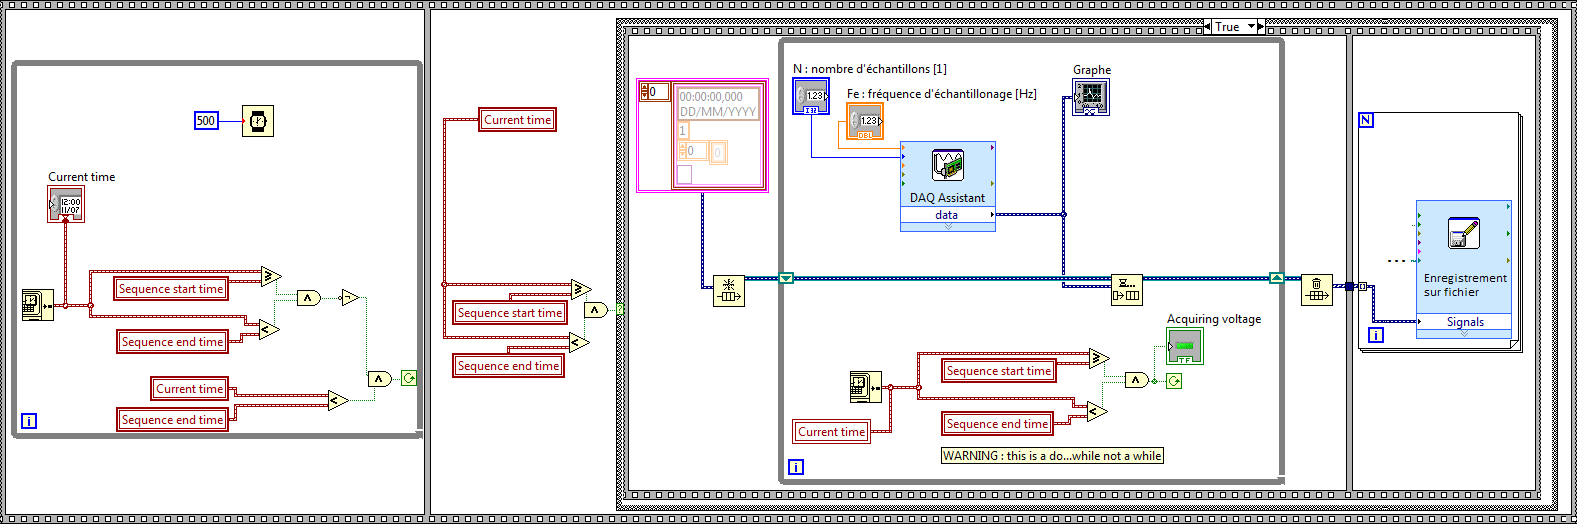
\includegraphics[width=17.5cm]{pictures/minuterie.png}
\caption{Impl\'ementation de la minuterie en LabVIEW}
\label{fig:algo_timer_labview}
\end{figure*}

\begin{remark}
  \textsc{(pr\'ecision des d\'eclenchements et arr\^ets de s\'equences d'acquisition)}
  Soit $\varepsilon > 0$.
  Si l'on note $F_r$ la fr\'equence de rafra\^ichissement du logiciel, on risque d'avoir une erreur de retard d'acquisition de l'ordre de $\frac{1}{F_r} - \varepsilon$. La boucle d'acquisition v\'erifie le temps initial \`a p\'eriode $\Delta t$ (largeur de fen\^etre de calcul). On risque alors d'avoir une erreur de d\'epassement de temps d'acquisition \`a $\Delta t - \varepsilon$ pr\`es. 
\end{remark}

\subsection{Boucle d'acquisition}

\noindent
\textbf{Technique.} Le temps d'\'echauffement recommand\'e du bo\^itier d'acquisition avant usage est de $15$ minutes\cite{NI_6353_datasheet}.

\begin{definition}
  (\textsc{boucle d'acquisition})
  Une \textit{boucle d'acquisition} est une structure de contr\^ole permettant l'acquisition r\'ep\'et\'ee et cadenc\'ee des valeurs retourn\'ees par le bo\^itier d'acquisition \`a un instant $t$ durant un temps fini $\Delta t$ \`a une fr\'equence $F_e$.
\end{definition}

Une s\'equence d'acquisition est r\'ealis\'ee par une boucle d'acquisition (\textsc{algorithme}~\ref{algo_boucle_acquisition}) qui appelle la fonction \texttt{DAQ Assistant}~\ref{fig:NI_DAQ_Assitant}~\cite{NI_acquisition_design_ref}~\cite{NI_Dynamic_data} et stocke les valeurs retourn\'ees en m\'emoire morte.

%~\cite{MSDN_memory}~\cite{NI_extend_memory}~\cite{NI_deallocation}

\begin{remark}
  Une minimisation des temps de retards impos\'es par les limitations physiques du disque dur est rendue optimale par la m\'emoire tampon du bo\^itier d'acquisition\cite{NI_6353_datasheet} sans intervention de l'utilisateur.
\end{remark}

\begin{algorithm}[h]
\caption{Boucle d'acquisition}
\label{algo_boucle_acquisition}
\begin{algorithmic}[1]
  \REQUIRE $t_i()$ : temps initial, $t_d$ : temps de d\'ebut d'acquisition, $t_f$ : temps de fin
  \STATE $F$ : fichier
  \WHILE {$t_d \leq t_i() < t_f$}
  \STATE $F \Leftarrow$ \texttt{acqu\'erir}()
  \ENDWHILE
  \RETURN $F$
\end{algorithmic}
\end{algorithm}

\subsection{\'Echantillonage}
On se propose d'introduire quelques notations permettant de clarifier les prochaines configurations.

\begin{notation}
Soit $x : I \rightarrow \mathbb{R}, t \mapsto x(t)$ un signal \`a $N$ \'echantillons index\'es par $I$. On note :
\begin{description}
\item[$F_c$]{ : la fr\'equence centrale [Hz]}
\item[$\Delta f$]{ : la largeur de bande passante [Hz]}
\item[$F_e$]{ : la fr\'equence d'\'echantillonage [Hz]}
\item[$F_b$]{ : le d\'ebit binaire du signal modul\'e [Hz = $\operatorname{bits}.\operatorname{s}^{-1}$]}
\item[$N$]{ : le nombre d'\'echantillons [1]}
\item[$\Delta t$]{ : la largeur de fen\^etre de calcul [s]}
\end{description}
\end{notation}

%\begin{notation}
%\begin{equation}
%  \Delta t = \frac{N}{F_e}
%\end{equation}
%\end{notation}

\begin{figure}[h]
  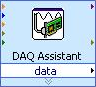
\includegraphics[width=2.5cm]{pictures/DAQ_Assistant.png}
\caption{Fonction \texttt{DAQ Assistant}}
\label{fig:NI_DAQ_Assitant}
\end{figure}

\noindent
\textbf{Configuration.} Lors de la d\'efinition de la fonction \texttt{DAQ Assistant}, les param\`etres suivants correspondent aux valeurs d\'efinies plus haut :
\begin{itemize}
  \item{\texttt{Acquisition mode} : choisir \texttt{Continuous Samples}}~\cite{NI_continuous_samp}
  \item{\texttt{Samples to Read} : $N$}
  \item{\texttt{Rate (Hz)} : $F_e$}
\end{itemize}

\begin{remark}
  (\textsc{m\'emoire tampon fifo du bo\^itier})
  Le bo\^itier poss\`ede une m\'emoire tampon \textsc{fifo} de $4095$ \'echantillons~\cite{NI_6353_datasheet} (csq ?).
\end{remark}

\begin{remark}
  \textsc{(complexit\'e)}
  Le co\^ut en temps de la fonction \texttt{DAQ Assistant} s'exprime en $\Omega(N)$\cite{omega} et prend un temps $\Delta t = \frac{N}{F_e}$ entre l'appel de fonction et le retour des valeurs.
\end{remark}

La largeur de fen\^etre choisie est de $\frac{1}{F_b}$ (pk?).

On justifie dans les paragraphes suivants les choix de configurations d'\'echantillonage optimaux pour l'acquisition.

\begin{theorem} (\textsc{Nyquist-Shannon}~\cite{Nyquist}~\cite{Shannon})
  \begin{eqnarray}
    F_e \geq 2 \times \operatorname{max} \left \{ F_c ; F_b \right \}
  \end{eqnarray}
\end{theorem}

\begin{remark}
  \textsc{(\'echantillonage optimal)}
  Le th\'eor\`eme \'enonce que, pour un signal num\'erique, la fr\'equence d'acquisition de base th\'eorique est de $0,5$ Hz par baud. En pratique, il faudrait au moins entre $0,7$ et $0,8$ Hz par baud\cite{FV}.
\end{remark}

Le bo\^itier d'acquisition \texttt{NI-6353} peut fournir une fr\'equence d'\'echantillonage de $1$ M\'ech./s sur plusieurs voies~\cite{NI_6353_datasheet}. L'acquisition de toutes les voies devant \^etre quasi-simulaltan\'ee, il para\^it trivial que toutes les voies soient au moins \'echantillon\'ees \`a $2 \times 2,4 \times 10^3 = 4,8 \times 10^3$ Hz (par application du th\'or\`eme pr\'ec\'edent). On note cependant que certains \textsc{dsp} ne se limitent qu'\`a $4 \times F_c$ pour des raisons de surcharge de calculs~\cite{TI_MSP430}.

En consid\'erant un post-traitement des op\'erations de nu\'erisation des signaux, on peut alors, pour des raisons de pr\'ecision de mesures, \'echantilloner chacune des voies \`a 10 kHz.

\subsection{D\'etection de composante fr\'equentielle et transform\'ee de Fourier}

{ \color{rltred}{\Radioactivity} } Cette partie n'entre en aucune consid\'eration dans le plan logiciel. Il n'est qu'une justification quant \`a l'usage des d\'emodulateurs de fr\'equence pourvus par les quatre transceivers \texttt{VR-5000}. Cette derni\`ere assure les op\'erations de calcul d'amplitudes associ\'ees aux composantes fr\'equentielles d\'efinies plus haut, incluant nativement des tranformations de Fourier.

\begin{definition}
\textsc{(spectre fr\'equentiel)}
Soit $\mathcal{F}$ la transform\'ee de Fourier d'une fonction int\'egrable sur $\mathbb{R}$ et $\hat{x} = \mathcal{F}(x) = \left [ k \mapsto \hat{x}(k)\right ]$ le \textit{spectre fr\'equentiel} de $x$ au $k$-i\`eme \'echantillon. On a\cite{Senlis} :

\begin{eqnarray*}
\hat{x}(k) &=& \sum^{N - 1}_{n = 0}{x(n)e^{\frac{-2ik \pi n}{N}}}\\
           &=& \sum^{N - 1}_{n = 0}{x(n)\cos \left ( \frac{2k \pi n}{N} \right )} - i\sum^{N - 1}_{n = 0}{x(n)\sin \left ( \frac{2k \pi n}{N} \right )}
\end{eqnarray*}
\end{definition}

On note $A (f)$ l'amplitude de la composante fr\'equentielle $f$.

\begin{proposition}
\textsc{(amplitude)}
La transform\'ee de Fourier d'un signal \`a $N$ \'echantillons est une application qui \`a un indice $k$ ($k \in [0 ; N - 1]$) associe le spectre de la fr\'equence $f$ tel que $f = \frac{k.F_e}{N}$.
\end{proposition}

On a alors que\cite{Senlis} :
\begin{eqnarray*}
  A (f) &=& \left \| \hat{x} \left (\frac{f.N}{F_e} \right ) \right \|\\
           &=& \sqrt{\mathfrak{Re} \left ( \hat{x} \left (\frac{f.N}{F_e} \right ) \right )^2 + \mathfrak{Im} \left ( \hat{x} \left (\frac{f.N}{F_e} \right ) \right )^2}
\end{eqnarray*}

\subsection{D\'emodulation \texttt{FSK}}

En consid\'erant que les op\'erations de d\'emodulation \texttt{FSK} sont r\'ealis\'ees par le transceiver \texttt{VR5000}, on propose l'algorithme suivant afin de num\'eriser les amplitudes associ\'ees aux composantes fr\'equentielles d'un signal \`a partir d'une liste de $N$ mesures de tensions.

\begin{proposition}
  \textsc{(\'echantillons)}
  Sachant que l'on souhaite d\'etecter la pr\'esence du \texttt{1} ou du \texttt{0} logique sur un temps $\Delta t = \frac{1}{F_b}$. On a :
  \begin{eqnarray}
    N = \frac{F_e}{F_b}
  \end{eqnarray}

L'algorithme suivant doit alors \^etre ex\'ecut\'e sur un signal \`a $\frac{F_e}{F_b}$ valeurs.
\end{proposition}

\noindent
\textbf{Id\'ee.}
\textsc{(num\'erisation fsk)}
  On cherche, \`a partir d'un signal compos\'e de deux amplitudes, \`a distinguer celle ayant l'occurence la plus r\'eguli\`ere. On peut alors calculer la moyenne du signal et v\'erifier si cette valeur ``se rapproche plus'' d'une amplitude ou d'une autre autre.

On propose un algorithme (\textsc{algorithme}~\ref{algo_numerisation_FSK}, \textsc{impl\'ementation~\ref{fig:algo_numerisation_FSK_labview}}) qui ne d\'etecte qu'un seul bit d'information par signal $x$ re\c{c}u et qui, \`a partir de deux amplitudes $A(f_0)$ et $A(f_1)$, renvoie la num\'erisation de $x$ comme suit:
  \begin{eqnarray*}
    \texttt{numerisation\_FSK} (x) =\\
    \left\{\begin{matrix}
    \texttt{0} &\textup{si }& \left | \operatorname{moyenne}(x) - A(f_0) \right | > \left | \operatorname{moyenne}(x) - A(f_1) \right |\\ 
    \texttt{1} &\textup{sinon}&
    \end{matrix}\right.
  \end{eqnarray*}

\begin{proposition}
  \textsc{(formule de la moyenne)}
  Soient $N \in \mathbb{N}$ et $f : \left \{ 0 ; \dots ; N - 1 \right \} \rightarrow \mathbb{R}$ un signal \`a $N$ \'echantillons. On d\'efinit la moyenne du signal $f$ par la fonction :
  \begin{eqnarray*}
    \mathbb{R}^{\left \{ 0 ; \dots ; N - 1 \right \}} &\rightarrow& \mathbb{R}\\
    \operatorname{moyenne} : f &\mapsto& \frac{1}{N}\sum^{N - 1}_{i = 0}{f(i)}
  \end{eqnarray*}
\end{proposition}

\noindent
\textbf{Sp\'ecification.}
  Lors de l'\'ecriture des bits de donn\'ees, la d\'etection de l'amplitude associ\'e \`a la composante $f_0$ (combien?) indique le \texttt{0} logique tandis que celle associ\'ee \`a $f_1$ (combien?) indique le \texttt{1}~\cite{Comment1}.

\begin{algorithm}[h]
\caption{Num\'erisation FSK}
\label{algo_numerisation_FSK}
\begin{algorithmic}[1]
  \REQUIRE signal $x$ \`a $N$ valeurs, amplitude de $f_0$ : $A(f_0)$ et amplitude de $f_1$ : $A(f_1)$
  \STATE $\texttt{moyenne} \leftarrow \frac{1}{N}\sum^N_{i = 0}{x(i)}$
  \IF {$\left | \texttt{moyenne} - A(f_0) \right | > \left | \texttt{moyenne} - A(f_1) \right |$}
  \RETURN \texttt{0}
  \ELSE
  \RETURN \texttt{1}
  \ENDIF
\end{algorithmic}
\end{algorithm}


\begin{figure*}[]
  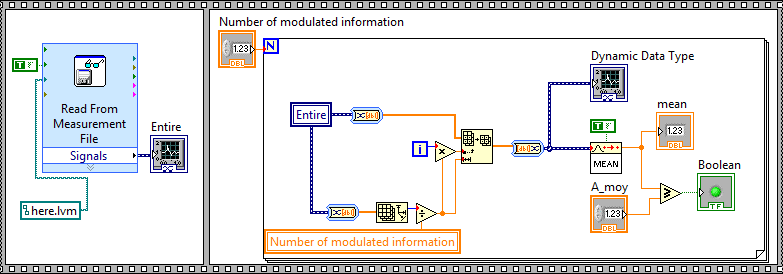
\includegraphics[width=15cm]{pictures/numerisation_amplitude.png}
\caption{Impl\'ementation du num\'erisateur d'amplitudes en LabVIEW}
\label{fig:algo_numerisation_FSK_labview}
\end{figure*}

%\begin{remark}
%  Lors de l'\'ecriture des bits de donn\'ees, la d\'etection de la composante $F_c + \frac{\Delta f}{2}$ indique la n\'gation du bit pr\'ec\'edent tandis que $F_c - \frac{\Delta f}{2}$ indique le bit similaire au pr\'ec\'edent.
%\end{remark}

%\begin{definition}
%  Soient $x$ un signal de largeur de fen\^etre de calcul $\Delta t = \frac{1}{F_b}$ et $\mathbb{B} = \{\texttt{0}, \texttt{1}\}$ un alphabet. On appelle $\delta : \mathbb{R}^{I} \rightarrow \mathbb{B}$ la fonction de \texttt{FSK}-d\'emodulation de $x$. Alors:
%\begin{eqnarray}
%  \delta (x) = \left\{\begin{matrix}
%&\texttt{0}& \textup{si} \ A (F_c - \frac{\Delta f}{2}) > A (F_c + \frac{\Delta f}{2})\\ 
%&\texttt{1}& \textup{sinon}
%\end{matrix}\right.
%\end{eqnarray}
%\end{definition}

\subsection{D\'emodulation OOK (CW)}

La modulation en \textit{On-Off Keying} (OOK) est un cas particulier de la modulation en \texttt{ASK} (Amplitude Shift-Keying). Les donn\'ees num\'eriques sont modul\'ees par la pr\'esence ou bien l'abscence du signal porteur $F_c$. On note $A(F_c)$ l'amplitude associ\'ee \`a la composante fr\'equentielle $F_c$. De mani\`ere analogue, en consi\'erant que les op\'rations de d\'emodulation sont effectu\'ees par le \texttt{VR5000}, on propose un algorithme (\textsc{algorithme}~\ref{algo_numerisation_OOK}) similaire de num\'erisation de donn\'ees modul\'ees en \texttt{OOK}.

\begin{algorithm}[h]
\caption{Num\'erisation OOK}
\label{algo_numerisation_OOK}
\begin{algorithmic}[1]
  \REQUIRE signal $x$ \`a $N$ valeurs, amplitude de $F_c$ : $A(F_c)$
  \IF {$\frac{1}{N}\sum^{N}_{i = 0}{x(i)} < \frac{A(F_c)}{2}$}
  \RETURN \texttt{0}
  \ELSE
  \RETURN \texttt{1}
  \ENDIF
\end{algorithmic}
\end{algorithm}

\subsection{D\'ecodage de trames AX.25 et automates finis}

\begin{definition}
  { \color{rltred}{\Radioactivity} }
  \textsc{(lsb$-$msb)}
  Soit $x$ un nombre binaire. Il existe alors une suite finie $\left ( b_n \right )_{0 \leq n \leq n_0}$ d'entiers \'egaux \`a $0$ ou $1$ tel que
  \begin{eqnarray*}
    x = \sum^{n_0}_{n = 0}{b_n \times 2^n}
  \end{eqnarray*}
  L'entier $b_0$ est appel\'e \textit{bit de poids faible} (\textsc{lsb}) et l'entier $b_{n_0}$ le \textit{bit de poids fort} (\textsc{msb}).
\end{definition}

\begin{example}
  On pose $x$ le nombre $42$ en repr\'esentation d\'ecimale, on note $(x)_{\textup{bin}}$ la repr\'sentation binaire de $x$ dans la notation positionelle habituelle, on a :
\begin{eqnarray*}
  (x)_{\textup{bin}} = \underbrace{1}_{\textup{MSB}}0101\underbrace{0}_{\textup{LSB}}
\end{eqnarray*}

\begin{comment}
\begin{figure}[h]
  \begin{tabular}{|c|}
    \hline
    $\dots$
    \textcolor{rltred}{$\underbrace{\texttt{01111110}}_{\textup{debut de trame}}$}
    $\dots$
    \textcolor{rltgreen}{$\underbrace{\texttt{10101010}}_{\textup{information}}$}
    $\dots$
    \textcolor{rltred}{$\underbrace{\texttt{01111110}}_{\textup{fin de trame}}$}
    $\dots$\\
    \hline
  \end{tabular}
\caption{Bits de donn\'ees correspondant au signal modulant}
\label{fig:geometry}
\end{figure}
\end{comment}

\end{example}

\begin{remark}
  (\textsc{boutisme de bits})
  Tous les octets (mots de longeur 8) d'une trame AX.25 (except\'e pour le facteur FCS) sont re\c{c}us avec le \textit{bit de poids faible} en premier\cite{IITB}. Le facteur FCS d'une telle trame est la concat\'enation d'octets de poids forts en premier.
\end{remark}

On note l'alphabet $\mathbb{B} = \{\texttt{0}, \texttt{1}\}$.

\begin{definition}
  \textsc{(trame ax.25 de pratham)}
  Un mot $m$ sur l'alphabet $\mathbb{B}$ est une \textit{trame AX.25 de Pratham}~\cite{IITB}~\cite{ax25} s'il est la concat\'enation des facteurs suivants (\`a un facteur \textit{fanion} pr\`es):
  \begin{footnotesize}
    \begin{tabular}{|c|c|c|c|c|c|c|}
      \hline
      \multicolumn{7}{|c|}{$m$ : 114 octets}\\
      \hline
      Fanion & Adresse & Contr\^ole & PID & {\tiny Information} & FCS & Fanion\\
      \hline
      $\texttt{01111110}$ & $\dots$ & $\texttt{00000011}$ & $\texttt{11110000}$ & $\dots$ & $2$ octets & $\texttt{01111110}$\\
      \hline
    \end{tabular}
  \end{footnotesize}
\begin{center}
  \begin{footnotesize}
    \begin{tabular}{|c|c|c|c|c|c|c|c|}
      \hline
      \multicolumn{8}{|c|}{Adresse : 21 octets}\\
      \hline
      \multicolumn{3}{|c|}{Sous-adresse$_1$} & \multicolumn{2}{c|}{Sous-adresse$_2$} & \multicolumn{3}{c|}{Sous-adresse$_3$}\\
      \hline
      \multicolumn{3}{|c|}{7 octets} & \multicolumn{2}{c|}{7 octets} & \multicolumn{3}{c|}{7 octets}\\
      \hline
      \texttt{CQ} & $\left ( (20)_{\operatorname{hex}} \right )^4$ & \texttt{01100000} & \texttt{VU2DMQ} & \texttt{01100000} & \texttt{RELAY} & $(20)_{\operatorname{hex}}$ & \texttt{01100000}\\
      \hline
    \end{tabular}
  \end{footnotesize}
\end{center}

\begin{center}
  \begin{footnotesize}
    \begin{tabular}{|c|}
      \hline
      Information : 87 octets\\
      \hline
      \textit{Health monitoring data}\cite{IITB}\\
      \hline
    \end{tabular}
  \end{footnotesize}
\end{center}

\end{definition}

\begin{theorem}
  { \color{rltred}{\Radioactivity} }
  \textsc{(Kleene)} Soit un alphabet fini $\Sigma$.
  \begin{eqnarray*}
    \operatorname{Rat} \Sigma^{\star} = \operatorname{Rec} \Sigma^{\star} 
  \end{eqnarray*}
\end{theorem}

\begin{proposition}
  { \color{rltred}{\Radioactivity} }
  Soit $e$ une expression rationnelle d\'enotant un langage $L(e)$ sur l'alphabet $\mathbb{B}$ tel que :
  \begin{eqnarray}
    \exists u \in \mathbb{B}^{\star} \ \forall w \subset u \
    \left\{\begin{matrix}
        e &=& (\texttt{01111110}) . u . (\texttt{01111110})^{\star}\\ 
        w &\neq& \texttt{01111110}
      \end{matrix}\right.
  \end{eqnarray}
Il existe un automate fini $A$ tel que $A$ reconnaisse $L (e)$.
\end{proposition}

\begin{remark}
  (\textsc{syntaxe des trames Pratham en AX.25})
  La syntaxe des trames du protocole AX.25 est pr\'esent\'ee en \textsc{figure}~\ref{fig:EBNF_ax25} afin d'impl\'ementer un analyseur syntaxique.
\end{remark}

\begin{figure*}
{\scriptsize
\begin{verbatim}
AX.25 packets protocol
--------
packets     ::= { frame }
frame       ::= flag+ address control pid information fcs flag
flag        ::= "01111110"
address     ::= "CQ" ((20)_hex)^4 "01100000" "VU2DMQ" "01100000" "RELAY" (20)_hex "01100000" (* à retranscrire *)
control     ::= "00000011"
pid         ::= "11110000"
information ::= (* pratham *)
fcs         ::= (* attention au boutisme *)
\end{verbatim}
}
\caption{Syntaxe des trames Pratham en AX.25 en notation EBNF}
\label{fig:EBNF_ax25}
\end{figure*}


\begin{implementation}
  (\textsc{algorithme~\ref{algo_decoupage_trames_ax25}})
  { \color{rltred}{\Radioactivity} }
  On proc\`ede \`a une analyse lexicale sur les bits de donn\'ees, d'o\`u l'int\'er\^et et l'usage d'automates finis, afin de d\'ecouper les trames s\'epar\'ees par des fanions. On impl\'emente un analyseur lexical munie d'une file\cite{Comment2}~\cite{Knuth} avec \texttt{ocamllex}~\cite{ocaml_parsing}.
\end{implementation}

\begin{algorithm}[h]
\caption{D\'ecoupage de trames AX.25}
\label{algo_decoupage_trames_ax25}
\begin{algorithmic}[1]
  \REQUIRE mot $m = m_0 \dots m_{p  - 1}$ sur l'alphabet $\mathbb{B}$ de longueur $p$
  \STATE mot vide $a$ \hfill //\textit{accumulateur indiquant l'ouverture ou non d'une nouvelle trame}
  \STATE liste vide $l$
  \STATE \textbf{analyse lexicale} de $m$ \textbf{faire}
  \STATE \textbf{parse} \texttt{01111110} :
  \IF {une trame n'est pas ouverte}
  \STATE ouvrir une nouvelle
  \ELSE
  \IF {une trame est d\'ej\`a ouverte,}
  \IF {elle n'est pas vide}
  \STATE la refermer et l'enfiler dans $l$
  \ENDIF
  \ENDIF
  \ENDIF
  \STATE \textbf{parse} \texttt{\_} :
  \IF {une trame est d\'ej\`a ouverte}
  \STATE {concat\'ener le bit \texttt{\_} dans la trame}
  \ELSE
  \STATE ne rien faire \hfill \textit{//bits perdus car aucune trame ouverte}
  \ENDIF
  \STATE \textbf{fin analyse lexicale}
  \RETURN liste $l$ de mots binaires dont chaque \'el\'ement est une trame
\end{algorithmic}
\end{algorithm}

\begin{remark}
  \textsc{(bourrage de bit)}
  Le fanion \texttt{01111110} (\texttt{7E} hexad\'ecimal) ne peut donc, en aucun cas, avoir d'occurence dans de trames compl\`etes\cite{IITB}. Le proc\'ed\'e de \textit{bourrage de bit} (\textit{bit stuffing}) permet alors d'eviter la confusion entre les donn\'ees et les fanions. Durant la r\'eception des donn\'ees, on ignore le bit \texttt{0} \`a chaque occurence de cinq bits \text{1} cons\'ecutifs, apr\`es les op\'erations de d\'ecoupages de trames.
\end{remark}

\begin{implementation}
  (\textsc{algorithme~\ref{algo_extract_bit_stuffing}})
  { \color{rltred}{\Radioactivity} }
  Apr\`es le d\'ecoupage des trames, on extrait, de chaque trame, les bits de bourrage.
\end{implementation}

\begin{algorithm}[h]
\caption{Extraction du bit de bourrage}
\label{algo_extract_bit_stuffing}
\begin{algorithmic}[1]
  \REQUIRE mot $m = m_0 \dots m_{p  - 1}$ sur l'alphabet $\mathbb{B}$ de longueur $p$, $\cdot . \cdot$ la concat\'enation de deux mots
  \STATE mot vide $m'$
  \STATE compteur $c \leftarrow 0$
  \FOR {$i$ de $0$ \`a $p$}
  \IF {$m_i = 0$}
  \IF{$c = 5$}
  \STATE $c \leftarrow 0$
  \ELSE
  \STATE $c \leftarrow 0$
  \STATE $m' \leftarrow m'.0$    
  \ENDIF
  \ELSE
  \STATE $c \leftarrow c + 1$
  \STATE $m' \leftarrow m' . 1$
  \ENDIF
  \ENDFOR
  \RETURN $m'$
\end{algorithmic}
\end{algorithm}

\begin{implementation}
  (\textsc{algorithme~\ref{algo_decodage_ax25}})
  { \color{rltred}{\Radioactivity} }
  En consid\'erant que chaque unit\'e de trame, n'a pas le m\^eme boutisme de bits, on peut alors d\'ecouper les unit\'es \texttt{Adresse}, \texttt{Contr\^ole}, \texttt{PID}, \texttt{Information}, \texttt{FCS} et calculer leur repr\'esentation suivant la sp\'ecification \'etablie.
\end{implementation}

\begin{algorithm}[h]
\caption{Pattern-matching on AX.25 packets}
\label{algo_decodage_ax25}
\begin{algorithmic}[1]
  \REQUIRE liste de mots $l$
\end{algorithmic}
\end{algorithm}


\subsection{D\'ecodage du Morse}

\textbf{Liaison.} Simplex (d\'efinition \textsc{ansi})

\vspace{0.3cm}

\textbf{Sp\'ecification.}
La sp\'ecification du code Morse en vigueur dans le cadre du projet est celle d\'ecrite par l'International Telecommunication Union~\cite{ITU_morse}. On en rappelle ci-dessous la description :

\begin{enumerate}
  \item{La lettre \textsc{dah} ($-$) dure trois fois plus longtemps que la lettre \textsc{dit} ($\cdot$) ;}
  \item{L'\'ecart entre deux \'el\'ements (\textsc{dit} ou \textsc{dah}) d'une m\^eme lettre dure un \textsc{dit} ;}
  \item{L'\'ecart entre deux lettres d'alphabet dure un \textsc{dah} ;}
  \item{L'\'ecart entre deux mots dure sept \textsc{dit}.}
\end{enumerate}

\begin{definition}
  On note $\mathbb{M}$ l'alphabet Morse. On a :
  \begin{eqnarray*}
    \mathbb{M} = \left \{ \varepsilon_1, \varepsilon_3, \varepsilon_7, ., - \right \}
  \end{eqnarray*}
\end{definition}

\begin{definition}
  On d\'efinit par cas sur $\mathbb{M}$ l'application :
  \begin{eqnarray*}
    h : \mathbb{M} &\rightarrow& \mathbb{B^{*}}\\
                 m &\mapsto&
                 \left\{\begin{matrix}
                        \texttt{0} \ &\textup{si}& \ m &=& \varepsilon_1 \\ 
                        \texttt{000} \ &\textup{si}& \ m &=& \varepsilon_3 \\
                        \texttt{0000000} \ &\textup{si}& \ m &=& \varepsilon_7 \\
                        \texttt{1} \ &\textup{si}& m &=& \cdot\\
                        \texttt{111} \ &\textup{si}& m &=& -
                        \end{matrix}\right.
  \end{eqnarray*}
\end{definition}

\begin{definition}
On d\'efinit sur $\mathbb{M}$ la longueur d'une lettre $x \in \mathbb{M}$ comme \'etant l'application :
\begin{eqnarray*}
  L : \mathbb{M} &\rightarrow& \mathbb{N}\\
              x  &\mapsto&
                 \left\{\begin{matrix}
                 1 \ &\textup{si }& x &\in& \left \{ \texttt{.}, \varepsilon_1 \right \} \\
                 3 \ &\textup{si }& x &\in& \left \{ -, \varepsilon_3 \right \} \\ 
                 7 \ &\textup{si }& x &=& \varepsilon_7
              \end{matrix}\right.
\end{eqnarray*}
\end{definition}

\begin{proposition}
  {(\textsc{norme sur $\mathbb{M}^{\star}$})}
  Soit la fermeture de Kleene~\cite{kleene_star} de l'alphabet $\mathbb{M}$, not\'ee $\mathbb{M}^{\star}$. L'application
  \begin{eqnarray*}
    \widetilde{N} : \mathbb{M}^{\star} &\rightarrow& \mathbb{N}\\
    x = (x_0 \dots x_{n - 1}) &\mapsto& \sum_{i = 0}^{n - 1}{N(x_i)}
  \end{eqnarray*}
  est une norme sur $\mathbb{M}^{\star}$.
\end{proposition}

%utiliser mathcal
\begin{proof}
  Soit un mot $x \in \mathbb{M}^{\star}$. Il existe une suite de lettres de $\mathbb{M}$ $(x_1 \dots x_n)$ telle que 
  \begin{eqnarray*}
    x = (x_1 \dots x_n)
  \end{eqnarray*}
  \begin{enumerate}
    \item{(\textsc{s\'eparation})
      \begin{eqnarray*}
        \forall x \in \mathbb{M}^{\star}, \widetilde{N}(x) = 0 \Rightarrow x = \varepsilon
      \end{eqnarray*}
    }
    \item{(\textsc{homog\'en\'eit\'e})
      \begin{eqnarray*}
        \forall (\lambda, x) \in \mathbb{N} \times \mathbb{M}^{\star}, \widetilde{N}(x^{\lambda}) = \lambda \widetilde{N}(x)
      \end{eqnarray*}
    }
    \item{(\textsc{in\'egalit\'e triangulaire})
      \begin{eqnarray*}
        \forall (x, x') \in \mathbb{M}^{\star}, \widetilde{N}(x.x') \leq \widetilde{N}(x) + \widetilde{N}(x')
      \end{eqnarray*}
    }
  \end{enumerate}
\end{proof}

\begin{figure*}[]
  \begin{eqnarray*}
    \underbrace{\underbrace{\underbrace{\texttt{1}}_{.} \underbrace{\texttt{0}}_{\varepsilon_1} \underbrace{\texttt{1}}_{.}}_{I} \underbrace{\texttt{000}}_{\varepsilon_3} \underbrace{\underbrace{\texttt{1}}_{.} \underbrace{\texttt{0}}_{\varepsilon_1} \underbrace{\texttt{1}}_{.}}_{I} \underbrace{\texttt{000}}_{\varepsilon_3} \underbrace{\underbrace{\texttt{111}}_{-}}_{T}}_{IIT}
    \underbrace{\texttt{1111111}}_{\varepsilon_7}
    \underbrace{\underbrace{\underbrace{\texttt{111}}_{-} \underbrace{\texttt{0}}_{\varepsilon_1} \underbrace{\texttt{1}}_{.} \underbrace{\texttt{0}}_{\varepsilon_1} \underbrace{\texttt{1}}_{.} \underbrace{\texttt{0}}_{\varepsilon_1} \underbrace{\texttt{1}}_{.}}_{B} \underbrace{\texttt{000}}_{\varepsilon_3} \underbrace{\underbrace{\texttt{111}}_{-} \underbrace{\texttt{0}}_{\varepsilon_1} \underbrace{\texttt{111}}_{-} \underbrace{\texttt{0}}_{\varepsilon_1} \underbrace{\texttt{111}}_{-}}_{O} \underbrace{\texttt{000}}_{\varepsilon_3} \underbrace{\underbrace{\texttt{111}}_{-} \underbrace{\texttt{0}}_{\varepsilon_1} \underbrace{\texttt{111}}_{-}}_{M}}_{BOM}
  \end{eqnarray*}  
  \caption{Exemple des couches d'abstraction d'un signal Morse codant l'information \texttt{``IIT Bombay''}}
  \label{fig:exemple_signal_morse}
\end{figure*}


\begin{figure}[h]
  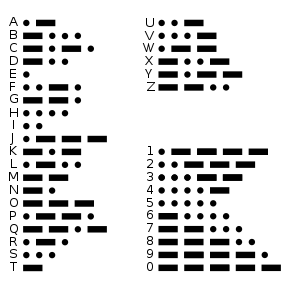
\includegraphics[width=6cm]{pictures/morse.png}
\caption{Alphabet du code Morse}
\label{fig:morse}
\end{figure}

\textbf{Impl\'ementation.} On impl\'emente tout d'abord un transducteur fini qui sur l'alphabet $\mathbb{B} = {\cdot, -}$ reconnait un mot sur $\mathbb{B}$ et retourne la lettre associee a son codage en Morse. Le transducteur est donn\'e en \textsc{figure} ~\ref{fig:transducteur_morse}.

\begin{figure*}
  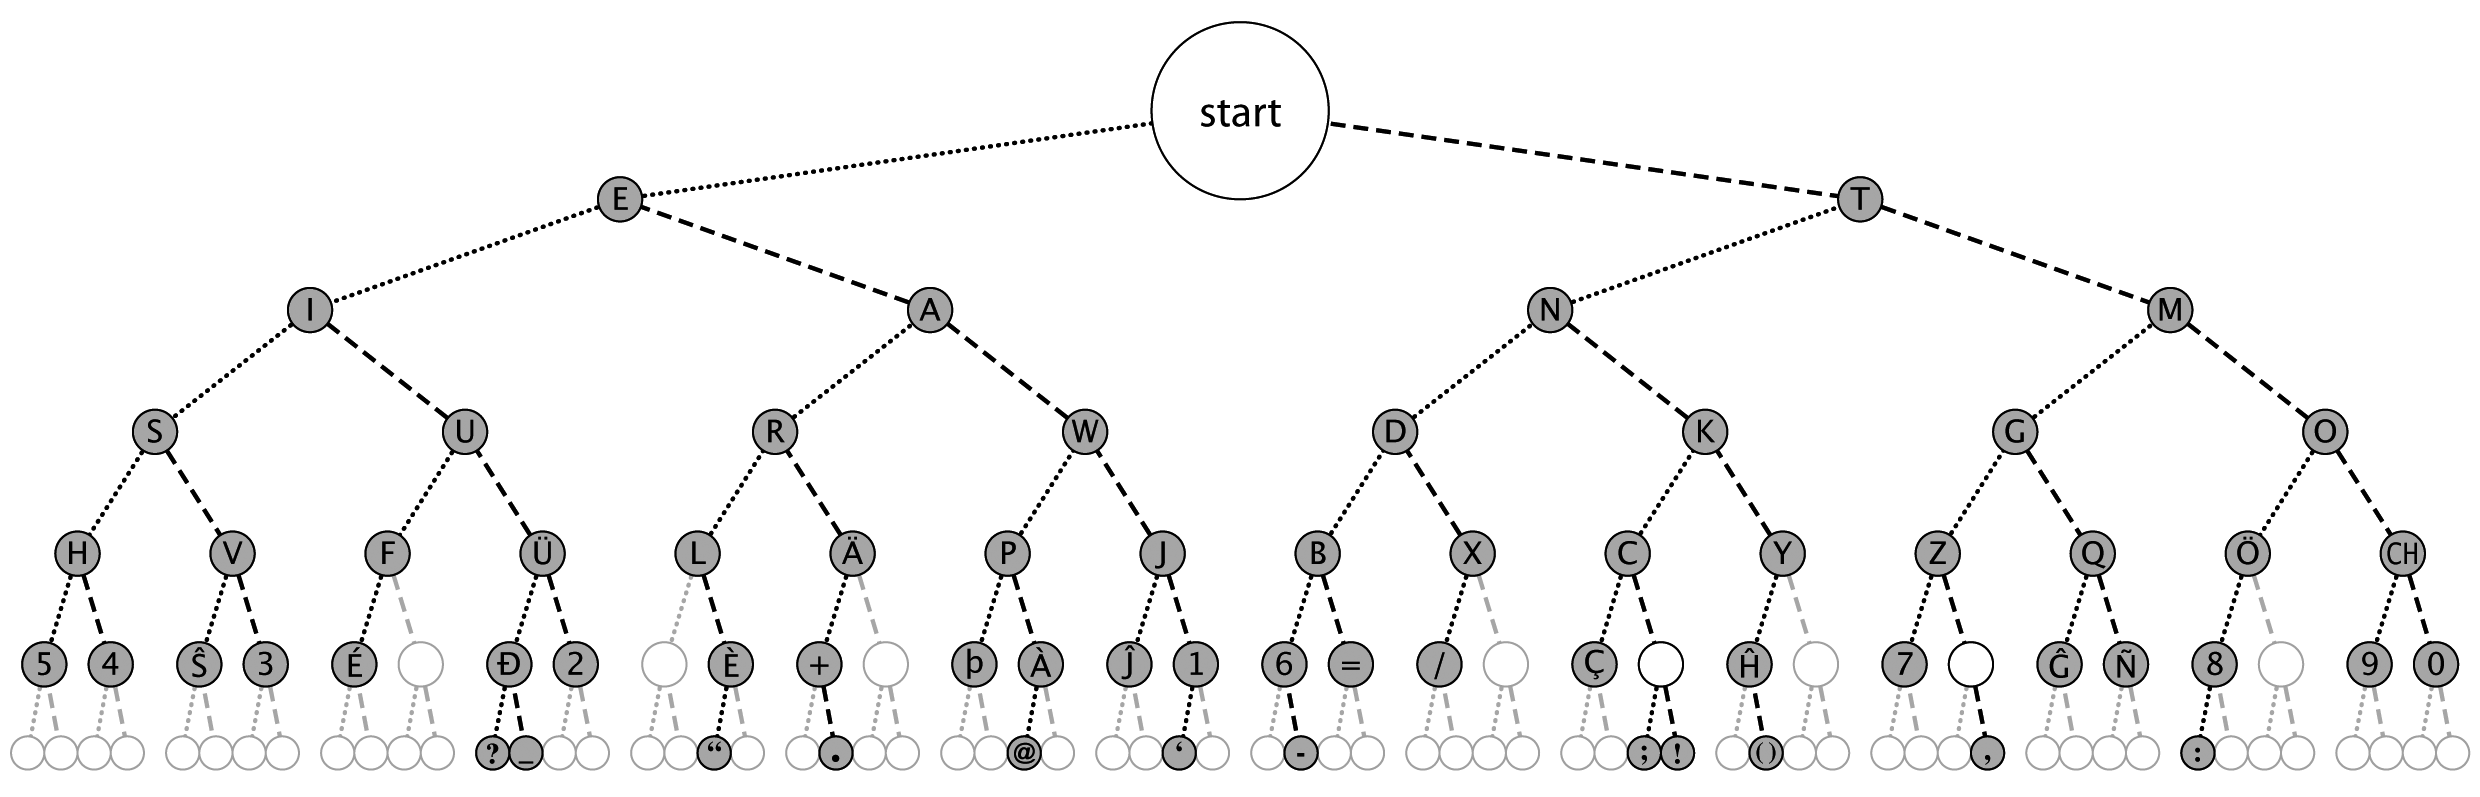
\includegraphics[width=17cm]{pictures/Morse_code_tree3.png}
\caption{Transducteur fini associ\'e au d\'ecodage \textsc{morse}~\cite{copyright_transducteur_morse}}
\label{fig:transducteur_morse}
\end{figure*}

\textbf{Impl\'ementation.} On termine l'implementation avec une analyse lexicale sur les bits issus de la num\'erisation du signal \`a $145,980$ MHz (\textsc{algorithme~\ref{lexing_signal_morse}}).

\begin{algorithm}[h]
\caption{D\'ecodage Morse \`a partir du signal modulant (num\'erique)}
\label{lexing_signal_morse}
\begin{algorithmic}[1]
  \REQUIRE mot $m = m_0 \dots m_{p  - 1}$ sur l'alphabet $\mathbb{B}$ de longueur $p$, transducteur $T_{\textup{Morse}}$ muni de \texttt{eval()}
  \STATE cha\^ine de caractr\`eres $acc$, et $res$ 
  \STATE \textbf{analyse lexicale} de $m$ \textbf{faire}
  \STATE \textbf{parse} \texttt{0000000} : \hfill \textit{(* $\varepsilon_7$ *)}
  \STATE $res \leftarrow res.$\texttt{`` ''}
  \STATE $acc \leftarrow \varepsilon$
  \STATE \textbf{parse} \texttt{000} : \hfill \textit{(* $\varepsilon_3$ *)}
  \STATE $res \rightarrow res .$ \texttt{eval}$(T_{\textup{Morse}}, acc)$
  \STATE $acc \leftarrow \varepsilon$
  \STATE \textbf{parse} \texttt{0} : \hfill \textit{(* $\varepsilon_1$ *)}
  \STATE $acc \leftarrow \varepsilon$
  \STATE \textbf{parse} \texttt{111} : \hfill \textit{(* $-$ *)}
  \STATE $acc \leftarrow acc . -$
  \STATE \textbf{parse} \texttt{1} : \hfill \textit{(* $\cdot$ *)}
  \STATE $acc \leftarrow acc . \cdot$
  \STATE \textbf{fin analyse lexicale}
  \RETURN $res$
\end{algorithmic}
\end{algorithm}

\subsection{Pr\'ecision de l'acquisition}
Le bo\^itier d'acquisition dispose d'un convertisseur analogique$-$num\'erique d'une r\'esolution de $16$ bits. La r\'esolution $Q$ du \textsc{can} ou \textit{tension du bit de poids faible} (\textsc{lsb}) est donn\'ee par la relation
\begin{eqnarray*}
  Q &=& \frac{E_{\textup{FSR}}}{N}\\
    &=& \frac{V_{\textup{RefHi}} - V_{\textup{RefLow}}}{2^M}
\end{eqnarray*}

o\`u :

\begin{description}
  \item[$E_{\textup{FSR}}$]{ : intervalle de tensions calibr\'es [V]}
  \item[$N$]{ : nombre d'intervalles de tensions [1]}
  \item[$V_{\textup{RefHi}}$]{ : calibre maximal de mesure de tension [V]}
  \item[$V_{\textup{RefLow}}$]{ : calibre minimal de mesure de tension [V]}
  \item[$M$]{ : r\'esolution du \textsc{can} [bit]}
\end{description}

La sp\'ecification du bo\^tier d'acquisition renseigne sur la pr\'ecision absolue~\cite{NI_6353_datasheet} en page ``AI Absolute Accuracy Table''.

On a alors d\'etermin\'e que nombre de chiffres significatifs de cet appareil de mesure s'\'el\`eve \`a 12 digits

\subsection{Enregistrement et sauvegarde des donn\'ees}

On r\'ealise une estimation des co\^uts en espace que peuvent engendrer l'enregistrement des valeurs de mesures au format de fichier Pratham en convention avec l'IITB\cite{IITB_filespec}. La dur\'ee d'acquisition lors d'un passage de satellite au$-$dessus de Paris d\'epend de plusieurs param\`etres, tels que :
\begin{itemize}
\item{l'altitude du satellite ;}
\item{le syst\`eme de tracking (\textsc{Nova}) :}
\item{l'ouverture de l'antenne ;}
\item{le multitrajet \`a basse \'el\'evation.}
\end{itemize}

On se propose d'effecuter une premi\`ere estimation sur les fichiers de donn\'ees brutes par intervalles de donn\'ees en portant \`a consid\'eration que 12 digits suffiront \`a la repr\'esentation des nombres \`a virgule flottante.

\begin{proposition}
  (\textsc{complexit\'e en espace d'un flottant})
  En consid\'erant que la repr\'esentation d'un nombre \`a virgule flottante en \textsc{ascii} s'effectue sur $12$ caract\`eres et qu'un caract\`ere en encodage \textsc{ascii} a un co\^ut en espace d'un octet. Alors un nombre \`a virgule flottante a un co\^ut en espace de $12$ octets.
\end{proposition}

\begin{remark}
  La repr\'esentation en machine 32$-$bits\cite{Alexandridis} suivant les conventions \textsc{ansi$-$c} d'un nombre sign\'e \`a virgule flottante en pr\'ecision simple ne co\^ute que 4 octets\cite{Marshall}, soit trois fois moins que la repr\'esentation pr\'ec\'edente.
\end{remark}

\begin{proposition}
  (\textsc{complexit\'e en espace des enregistrements de donn\'ees})
  Soit $(\mathbb{B}^{\star}, l_{\cdot})$ un espace norm\'e. On a alors l'approximation suivante de la longueur d'un enregistrement d'une s\'equence d'acquisition :
  \begin{eqnarray}
    l_{\textup{fichier}} &=& \underbrace{\Delta t}_{\in \left [ 7 ; 13 \right ] \ \operatorname{min}} \times \underbrace{f_e}_{10 \ \operatorname{kHz}} \nonumber\\
                    &\times& \underbrace{\left (\underbrace{l_{\textup{date}}}_{23 \ \operatorname{octets}} + \underbrace{n_{\textup{voies}}}_{12} \times (\underbrace{l_{\textup{flottant}}}_{12 \ \operatorname{octets}} + \underbrace{l_{\textup{separateur}}}_{1 \ \operatorname{octet}} ) \right )}_{\textup{une ligne}}\\
                    &\in& \left [ 7,518 \times 10^8 ; 1,3962 \times 10^9 \right ] \\
                    &\ &  \textup{car } \Delta t \mapsto l_{\textup{fichier}} (\Delta t) \ \textup{croissante} \nonumber
  \end{eqnarray}
\end{proposition}

En se basant sur une estimation du nombre de passages du satellite au dessus de Paris\cite{IPGP_simul_loic} :
\begin{eqnarray}
  n_{\textup{passages/jour}} \in \left [ 4 ; 6 \right ] \ \textup{passages}
\end{eqnarray}

On a alors par jour :

\begin{eqnarray}
  l_{\textup{jour}} &=& n_{\textup{passages/jour}} \times l_{\textup{fichier}}\\
                &\in& \left [ 3,0072 \times 10^9 ; 8,3772 \times 10^9 \right ] \\
                &\ & \textup{car } n_{\textup{passages/jour}} \mapsto l_{\textup{jour}} (n_{\textup{passages/jour}}) \ \textup{croissante} \nonumber
\end{eqnarray}

Sur un fonctionnement suppos\'e de 4 mois\cite{IITB_general} du satellite, il est n\'ecessaire de disposer d'un espace de stockage d'au moins :

\begin{eqnarray}
  l_{\textup{total}} &=& n_{\textup{passages/jour}} \times 30,5 \times 4 \times l_{\textup{fichier}}\\
                 &\in& \left [ 3,668784 \times 10^{11} ; 1,0220184 \times 10^{12} \right ]
\end{eqnarray}



On pr\'esente en \textsc{table}~\ref{tab:estimations_stockage}, les estimations de taille de fichier concernant les donn\'ees brutes à la sortie de l'acquisition.

\begin{table}[h]
  \caption{Estimations minimales et maximales de l'espace de stockage n\'ecessaire aux donn\'ees brutes}
  \begin{center}
    \begin{tabular}{@{\hspace{9pt}} c @{\hspace{9pt}} ||
        @{\hspace{6pt}} c @{\hspace{6pt}} | @{\hspace{6pt}} c
       @{\hspace{6pt}} }
      
      \hline\hline
      \multirow{2}{*}{Dur\'ee de temps (s)} & \multicolumn{2}{c}{Taille des fichiers {\hspace{9pt}} } \\
                                            & \textsc{min} & \textsc{max} \\ \hline
                                      1 min & \multicolumn{2}{c}{$107,4$ Mo} \\
                              1 seq. d'acq. & $751,8$ Mo & $1,4$ Go \\
                                     1 jour & $3,0$ Go & $8,37$ Go \\
                                     1 mois & $91,7$ Go & $255,5$ Go \\
                                     4 mois & $366,8$ Go & $1,02$ To \\
      \hline\hline

    \end{tabular}
  \end{center}
  \label{tab:estimations_stockage}
\end{table}

En consid\'erant que la fr\'equence d'\'echantillonage $F_e$ est de $10$ kHz, on obtient un instant de mesure
\begin{eqnarray*}
  T_e \stackrel{\mathrm{def}}{=} \frac{1}{F_e}
\end{eqnarray*}

Par passage de satellite, on n'obtient que 7200000 valeurs pour les slanTEC (calcul \`a justifier).

Dans le cadre d'une solution provisoire, on se permet d'utiliser le format de fichier de ``LabVIEW Measurement File''~\cite{NI_lvm} (\underline{solution \`a probleme car enregistre avec la date d'enregistrement et non la date d'acquisition}).

\subsection{Tol\'erance aux fautes}
Le syst\`eme de tol\'erance aux fautes se limite qu'\`a une gestion des exceptions par LabVIEW qui lors d'une exception poursuit l'acquisition et effectue un rapport.

\subsection{Logiciel final}

Le logiciel final sera compil\'e avec \texttt{NI Application Builder}~\cite{NI_compiler}~\cite{NI_application_builder}.

\section{Formats de fichier}
\label{sec:file_formats}

\subsection{\'El\'evations minimales/maximales fournies par Nova}

Nous donnons ci-dessous la syntaxe en EBNF des fichiers de donn\'ees sur les \'el\'evations minimales et maximales d'un satellite par rapport \'a un r\'ef\'erentiel g\'eographique.

LabVIEW, \'etant langage de programmation peu adap\'e \`a certains paradigmes, ne dispose pas de g\'en\'erateur d'analyseur syntaxique, ni lexical mais d'un analyseur par formats. Nous impl\'ementons provisoirement une analyse formatt\'ee avec la fonction \texttt{Scan From String}~\cite{NI_scan_from_string} (\textit{analyseur par formats d'une cha\^ine de caract\`eres \`a l'aide d'indicateurs de conversion}). On se propose de donner une preuve de correction de l'algorithme utilisant cet analyseur (\textsc{algorithme}~\ref{algo_scan_parse_nova}, \textsc{impl\'ementation}~\ref{fig:algo_scan_parse_nova_labview})~\cite{Knuth}.
%todo

\begin{algorithm}[h]
\caption{Analyse formatt\'ee des fichiers d'\'eph\'em\'erides de Nova}
\label{algo_scan_parse_nova}
\begin{algorithmic}[1]
  \REQUIRE $F$ : fichier
  \STATE hello world
  \RETURN $s$
\end{algorithmic}
\end{algorithm}

\begin{figure*}[]
  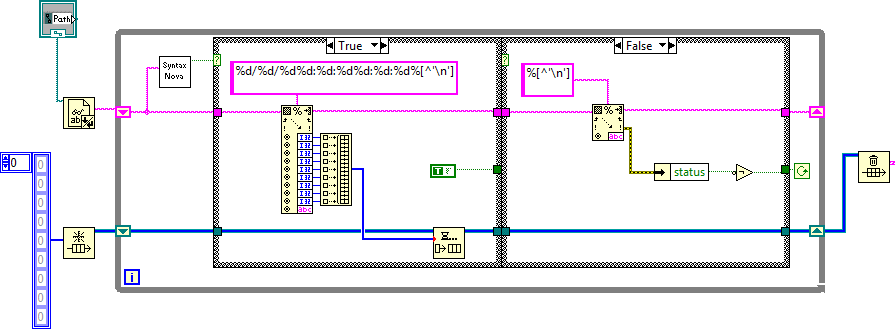
\includegraphics[width=17cm]{pictures/parser_nova_labview.png}
\caption{Impl\'ementation d'une analyse formatt\'ee en LabVIEW}
\label{fig:algo_scan_parse_nova_labview}
\end{figure*}

\begin{figure*}
\begin{verbatim}
Nova satellite AOS/LOS file
--------
file         ::= columns_desc { day_eclipses }

columns_desc ::= "Date (Z)" "AOS (Z)" "LOS (Z)" "Duration" "Between Az" '@' "AOS Max El Az" '@' "LOS Height" "km" newline

day_eclipses ::= day_header { day_entry }
day_header   ::= { character } "at" { character } ',' { character } newline
day_entry    ::= date time time time time int_number '°' int_number '°' int_number '°' float_number newline

date         ::= int_number '/' int_number '/' int_number
time         ::= int_number ':' int_number ':' int_number

newline      ::= \n
character    ::= 'a'|'b'|..|'A'|'B'|..|'0'|'1'|..
int_number   ::= [ '-' | '+' ] { '0' | .. | '9' }
float_number ::= [ '-' | '+' ] { '0' | ... | '9' } '.' { '0' | ... | '9' }
\end{verbatim}
\caption{Syntaxe des fichiers d'\'el\'evations minimales/maximales de Nova en notation EBNF}
\label{fig:EBNF_Nova}
\end{figure*}

\begin{figure*}
{\scriptsize
\begin{verbatim}

          Date (Z)           AOS (Z )  LOS (Z ) Duration  Between Az @ AOS Max El Az @ LOS Height  km 
ITUPSAT,1 at Paris ,France                                                                            
          16/04/12           10:55:23  11:05:03 00:09:40 01:01:01    38°     7°     126°      714.6   
          16/04/12           12:32:01  12:46:13 00:14:12 01:26:57    17°     58°    185°      714.6   
          16/04/12           14:10:15  14:23:00 00:12:43 01:24:02     4°     22°    236°      714.7   

\end{verbatim}
}
\caption{Exemple de fichier de pr\'evisions de passages de satellite produit par Nova}
\label{fig:EBNF_Nova2}
\end{figure*}

\subsection{Enregistrements Pratham}
Les formats de fichier qui seront utilis\'ees pour l'enregsitrement des donn\'ees de TEC vertical et slant sont sp\'ecifi\'ees dans le document ??? dont on donne une syntaxe en notation EBNF en ~\ref{fig:syntaxe_Pratham_format}.

\begin{figure*}[]
{\scriptsize
\begin{verbatim}
Raw output file from ground station acquisition (RAW_PRAT_SSSS_yyyy_ddd_hh_mm_ss.txt)
-------------------------
file ::= "Station_ID"             word
         "Location"               int_number ':' int_number ':' float_number int_number ':' int_number ':' float_number int_number
         "Satellite_Tracking_ID"  word
         "Start_time_UT"          time_stamp
         "End_time_UT"            time_stamp
         "Sampling_rate"          int_number
         "Data_points"            float_number
         "Acquisition_type"       int_number
         "Time" "145_VMAG1" "145_VPHS1" "145_VMAG2" "145_VPHS2" "437_VMAG1" "437_VPHS1" "437_VMAG2" "437_VPHS2"
         { time_stamp float_number float_number float_number float_number float_number float_number float_number float_number }

time_stamp   ::= int_number ':' int_number ':' int_number ':' int_number ':' int_number

word         ::= { character }
character    ::= 'a' | 'b' | ... | 'z' | 'A' | 'B' | ... | 'Z' | '0' | '1' | ... | '9'
int_number   ::= [ '-' | '+' ] { '0' | ... | '9' }
float_number ::= [ '-' | '+' ] { '0' | ... | '9' } '.' { '0' | ... | '9' }

\end{verbatim}
}
  \caption{Syntaxe des enregistrements au format Pratham en notation EBNF pour les donn\'ees brutes}
  \label{fig:syntaxe_Pratham_format}
\end{figure*}

Par souci de rigueur, on s'int\'eresse \`a la classe de grammaire \`a laquelle appartient la grammaire $G$ repr\'esentant cette syntaxe.

\begin{proposition}
  \begin{eqnarray*}
    G \in LL(1) 
  \end{eqnarray*} 
\end{proposition}

\begin{proof}
Montrons que la grammaire est $LL(1)$. Soit la grammaire $G$ dont le symbole de d\'epart est $F$ et dont on donne les ensembles de l\'ex\`emes en figure ~\ref{fig:LL1_pratham_analysis}. $D'$ est annulable.
  
On calcule $\text{FIRST}()$ et $\text{FOLLOW}()$ :
\begin{eqnarray*}
  \text{FIRST} (F)  &=& \{ \text{SI} \}\\
  \text{FIRST} (D)  &=& \{ n \}\\
  \text{FIRST} (L)  &=& \{ n \}\\
  \text{FIRST} (L') &=& \{ n, \dot{\epsilon} \}
\end{eqnarray*}
  
\begin{eqnarray*}
  \text{FOLLOW} (F) &=& \varnothing\\
  \text{FOLLOW} (S) &=& \{ f \}\\
  \text{FOLLOW} (D) &=& \{ \$ \}\\
  &\subseteq& \text{FOLLOW} (D') \text{ car } \dot{\epsilon} \in \text{FIRST} (D')\\
  \text{FOLLOW} (D') &=& \{ \$ \}
\end{eqnarray*}

Comme montr\'e en ~\ref{fig:LL1_pratham_analysis}, la grammaire ne pr\'esente aucun conflit FIRST/FIRST dans le cas d'une analyse $LL(1)$. Donc :

\begin{eqnarray*}
  G \in LL(1) 
\end{eqnarray*}
\hfill $\square$

\begin{figure*}
\begin{eqnarray*}
  \textup{Term} &=& \{ f, n, m, \$, SI, L, STID, STU, ETU, SR, DP, AT, T, 145_0, 145_1, 145_2, 145_3, 437_0, 437_1, 437_2, 437_3 \}\\
  \textup{NonTerm} &=& \{ F, S, D, D' \}
\end{eqnarray*}

\begin{eqnarray*}
  F  &\rightarrow& \text{SI} \ m \ \text{L} \ n : n : f \ n : n : n : f \ n \ \text{STI} \ m \ \text{STU} \ n : n : n : n : n  \ \text{ETU} \ n : n : n : n : n \  \text{SR} \ n \ \text{DP} \ f \ \text{AT} \ n\\
  && \text{T} \ 145_0 \  145_1 \  145_2 \  145_3 \ 437_0 \ 437_1 \ 437_2 \ 437_3 \ D \ \$ \\
  S &\rightarrow& n : n : n : n : n\\
  D  &\rightarrow& S \ f \ f \ f \ f \ f \ f \ f \ f  \ D'\\
  D' &\rightarrow& \epsilon | S \ f \ f \ f \ f \ f \ f \ f \ f \ D'
  \end{eqnarray*}


  \begin{center}
    \begin{tabular}{|c|c|c|c|c|c|c|c|c|c|c|c|c|c|c|c|c|c|c|c|c|c|}
      \hline
      & SI & L & STI & STU & SR & DP & AT & T & $145_0$ & $145_1$ & $145_2$ & $145_3$ & $437_0$ & $437_1$ & $437_2$ & $437_3$ & $f$ & $m$ & $n$ & : & \$\\
      \hline
      $F$  & $\{ F \rightarrow \dots \}$ & $\varnothing$ & $\varnothing$ & $\varnothing$ & $\varnothing$ & $\varnothing$ & $\varnothing$ & $\varnothing$ & $\varnothing$ & $\varnothing$ & $\varnothing$ & $\varnothing$ & $\varnothing$ & $\varnothing$ & $\varnothing$ & $\varnothing$ & $\varnothing$ & $\varnothing$ & $\varnothing$ & $\varnothing$ & $\varnothing$ \\
      \hline
      $S$  & $\varnothing$ & $\varnothing$ & $\varnothing$ & $\varnothing$ & $\varnothing$ & $\varnothing$ & $\varnothing$ & $\varnothing$ & $\varnothing$ & $\varnothing$ & $\varnothing$ & $\varnothing$ & $\varnothing$ & $\varnothing$ & $\varnothing$ & $\varnothing$ & $\varnothing$ & $\varnothing$ & $\{ S \rightarrow \dots \}$ & $\varnothing$ & $\varnothing$\\
      \hline
      $D$  & $\varnothing$ & $\varnothing$ & $\varnothing$ & $\varnothing$ & $\varnothing$ & $\varnothing$ & $\varnothing$ & $\varnothing$ & $\varnothing$ & $\varnothing$ & $\varnothing$ & $\varnothing$ & $\varnothing$ & $\varnothing$ & $\varnothing$ & $\varnothing$ & $\varnothing$ & $\varnothing$ & $\{ L \rightarrow \dots \}$ & $\varnothing$ & $\varnothing$\\
      \hline
      $D'$ & $\varnothing$ & $\varnothing$ & $\varnothing$ & $\varnothing$ & $\varnothing$ & $\varnothing$ & $\varnothing$ & $\varnothing$ & $\varnothing$ & $\varnothing$ & $\varnothing$ & $\varnothing$ & $\varnothing$ & $\varnothing$ & $\varnothing$ & $\varnothing$ & $\varnothing$ & $\varnothing$ & $\{ L' \rightarrow n \dots \}$ & $\varnothing$ & $\{ L' \rightarrow \epsilon \}$\\
      \hline
    \end{tabular}
  \end{center}
  \caption{Table d'analyse LL(1) de la grammaire}
  \label{fig:LL1_pratham_analysis}
\end{figure*}
\end{proof}

\section{Banc d'essai}
\label{sec:results}

\section{Preuves de programmes}
\label{sec:analysis}

{ \color{rltred}{\Radioactivity} }
Cette partie donne les preuves de correction des algorithmes mentionn\'es dans l'article. La m\'ethode formelle utilis\'ee sera la \textit{logique de Hoare}\cite{Hoare} (1969) et son cas particulier la preuve par \textit{invariant de boucle}.

\begin{definition}
  { \color{rltred}{\Radioactivity} }
  \textsc{(triplet de Hoare)}
  Soient $P$, $Q$ des pr\'edicats et \texttt{prog} un programme. Un triplet $T$ est un \textit{triplet de Hoare} si et seulement si
  \begin{eqnarray*}
    T = \{P\} \texttt{ prog } \{Q\}
  \end{eqnarray*}
\end{definition}

\begin{definition}
  { \color{rltred}{\Radioactivity} }
  \textsc{(correction d'un programme)}
  Un triplet de Hoare $\{P\} \texttt{ prog } \{Q\}$ est \textit{vrai} si pour tout \'etat initial v\'erifiant $P$, si l'ex\'ecution de \texttt{prog} termine, alors $Q$ est vraie apr\`es l'ex\'ecution de \texttt{prog}. Le programme \texttt{prog} est dit \textit{correct} par rapport \`a $P$ et $Q$.
\end{definition}

\subsection{Algorithme 1 : Minuterie}

\begin{proposition}
  L'algorithme d\'eclenche une suite de s\'equences d'acquisition $s_i$ \`a des temps pour chaque $s_i$. 
\end{proposition}

\begin{proof}
\end{proof}

\subsection{Algorithme 2 : Boucle d'acquisition}

\begin{proposition}
  L'algorithme boucle sur des acquisitions sur un temps fini $\Delta t$.
\end{proposition}

\begin{proof}
  Clair.
\end{proof}

\subsection{Algorithme 3 : Num\'erisation FSK}
\subsection{Algorithme 4 : Num\'erisation OOK}
\subsection{Algorithme 5 : D\'coupage de trames AX.25}
\subsection{Algorithme 6 : Extraction du bit de bourrage}
\subsection{Algorithme 7 : Pattern-matching on AX.25 packets}
\subsection{Informations sur la machine d'acquisition}

\subsection{Caract\'erisation du bo\^itier d'acquisition}



\begin{table}[h]
\caption{Force, area, and pressure data for the experiment shown in
Fig.~\ref{fig:geometry} and described by Eq.~\ref{eq:B}.  Agreement is
typically within five percent.}
\begin{center}
\begin{tabular}{l @{\hspace{30pt}} c @{\hspace{18pt}} c}
\hline\hline
& Piston 1 & Piston 2 \\ \hline
Avg. Force (N) & 4.40 & 2.25 \\
Area (cm$^2$) & 6.16 & 2.25 \\
$F/A$ (N/cm$^2$) & 0.714 & 0.717 \\
\hline\hline
\end{tabular}
\end{center}
\label{tab:pressure}
\end{table}

\section{Int\'egrit\'e et mise en route machine}

\subsection{Informations sur la machine}

Les logiciels suivants doivent \^etre install\'es et \'eventullement correctement configur\'es dans l'ordre\cite{NI_driver} suivant:
\begin{enumerate}
  \item{\href{http://digital.ni.com/src.nsf/websearch/968B3DF8AD48394D86257880005141A8?OpenDocument&node=node=203014_us}{LabVIEW 8.6 (National Instruments)}}
  \item{\href{http://joule.ni.com/nidu/cds/view/p/id/2260/lang/fr}{NI DAQ-mx 9.2.3 (pilote du bo\^itier d'acquisition)}}
  \item{\href{http://www.nlsa.com/uploads/nfw21v/nova_21v_download.html}{Nova for Windows 2.2c (NLSA)}}
  \item{\href{http://protz.github.com/ocaml-installer/}{OCaml 3.12 pour Windows}}
\end{enumerate}

Il sera pr\'evu que la machine d'acquisition $-$ pr\'evue pour fonctionner 24h/24 durant 4 mois $-$ sera de type :
\begin{itemize}
  \item{Mod\`ele : \href{http://support.dell.com/support/edocs/systems/latd630a/en/sm/index.htm}{Dell Latitude ATG D630}}
  \item{Processeur : \href{http://ark.intel.com/products/29761/Intel-Core2-Duo-Processor-T7500-\%284M-Cache-2_20-GHz-800-MHz-FSB\%29}{Intel Core 2 Duo T7500 (2,2 GHz, 2,19 GHz)}}
  \item{Syst\`eme d'exploitation : Microsoft Windows XP}
  \item{Disque dur : \href{http://storage.toshiba.com/storagesolutions/archived-models/mk8046gsx}{Toshiba MK8046GSX} (74,3 Go dont 71,5 Go occup\'es) (rapidit\'e d'\'ecriture ?)}
  \item{Carte r\'eseau :
    \begin{itemize}
      \item{LAN: \href{http://www.broadcom.com/support/ethernet_nic/netlink_k57.php}{Broadcom NetXtreme 57xx Gigabit Controller}}
      \item{Wifi: \href{http://www.intel.com/products/wireless/prowireless_mobile.htm}{Intel PRO/Wireless 3945 ABG Network Connection}}
    \end{itemize}
  }
\end{itemize}
\textsc{Dell Latitude atg D630}.

Elle sera constemment connect\'ee sur le r\'eseau afin de permettre \`a l'\'equipe de surveiller et de rapatrier les donn\'ees acquises.

\subsection{Syst\`eme d'avertissement et de gestion des erreurs}

\section{Conclusion}
\label{sec:conclusion}

\begin{thebibliography}{99}

\bibitem{cecill}Commissariat à l'Energie Atomique, Centre National de la Recherche Scientifique, Institut National de Recherche en Informatique et en Automatique, {\it \href{http://www.cecill.info/licences/Licence_CeCILL_V2-en.html}{CeCILL Free Software License Agreement}} (September, 2006)

\bibitem{IITB_general}Saptarshi Bandyopadhyay, Jhonny Jha, Haripriya, Ameya Damle, Deepika Thakur, Sanyam Mulay, Prashant Sachdeva, Jaideep Joshi, Vaibhav Unhelkar, Yashovardhan Chati, Mayank Chaturvedi, Niranjan Parab, Manas Rachh, Shashank Tamaskar, Mallesh Bommanahal, Ashish Goel, Kartavya Neema, Subhasis Das, Vishnu Sresht, Ramnath Pai, Ankit Chiplunkar, {\it \href{http://www.aero.iitb.ac.in/pratham/otherdocs/IIT-B_Paper_Pratham_20thApr.pdf}{Introduction to Pratham, IIT Bombay’s Student Satellite Project}} (IIT Bombay, June 2010)

\bibitem{IITB}J. Jha, S. Bandyopadhyay, C. Talnikar, {\it Pratham - Telemetry and Telecommand Document} (IIT Bombay, November 2010)

\bibitem{IITB_filespec}H. Nguyen Van, P. Co\"isson, P. Godbole, J. Jha, {\it Pratham satellite : File Formats Specification} (IPGP, May 2011)

\bibitem{IPGP_simul_loic}L. Viens, P. Co\"isson, {\it Pratham satellite : Paris Ground Station Simulations} (IPGP, November 2010)

\bibitem{Senlis}J. Senlis, {\it \href{http://jgsenlis.free.fr/dsp_28335.htm}{Formation DSP sur 320F28335}} (INSSET, Universit\'e de Picardie, 2008)

\bibitem{CHLS}T. Capitaine, M. Hamzaoui, A. Lorthois, J. Senlis, {\it \href{http://jgsenlis.free.fr/ax25/Cetsis2008_AX25.pdf}{D\'emodulation et d\'ecodage de trames AX.25 par DSPIC pour la localisation d'un ballon sonde m\'et\'eo dans le cadre d'une action ``Plan\`ete Sciences''}} (CETSIS, Bruxelles, 2008)

\bibitem{ax25}William A. Beech, Douglas E. Nielsen, Jack Taylor, {\it \href{http://www.tapr.org/pdf/AX25.2.2.pdf}{AX.25 Link Access Protocol for Amateur Packet Radio, version 2.2}} (Tucson Amateur Packet Radio Corporation, July 2008)

\bibitem{nova_um}Michael R. Owen, {\it \href{http://www.nlsa.com/docs/nfwdoc.pdf}{Nova for Windows $-$ User's Manual}} (Northern Lights Software Associates, February 2000)

\bibitem{Hoare}C. A. R. Hoare, {\it \href{http://www.spatial.maine.edu/~worboys/processes/hoare%20axiomatic.pdf}{An axiomatic basis for computer programming}} (Communications of the ACM 12 (10): 576-580)

\bibitem{FV}Agn\`es Foucher, Christian Valade, {\it \href{http://radiomods.free.fr/r2000-info/mod_dem_fsk.pdf}{Modulation, D\'emodulation, FSK. \'Etude structurelle}} (Universit\'e de Toulouse 1, F\'evrier 1999)

\bibitem{EBNF}International Organization for Standardization, {\it \href{http://standards.iso.org/ittf/PubliclyAvailableStandards/s026153_ISO_IEC_14977_1996(E).zip}{Information technology $-$ Syntactic metalanguage $-$ Extended BNF}} (ISO/IEC 141977, December 1996)

\bibitem{ITU_morse}International Telecommunication Union, {\it \href{http://www.itu.int/rec/R-REC-M.1677-1-200910-I/}{International Morse code $-$ Recommendation ITU-R M.1677-1}} (ITU, 2009)

\bibitem{NI_driver}National Instruments, {\it \href{http://www.ni.com/gettingstarted/installsoftware/dataacquisition.htm}{Install NI LabVIEW and NI-DAQmx Driver}} (2010)

\bibitem{NI_calibration_procedure}National Instruments, {\it \href{http://www.ni.com/pdf/manuals/370937k.pdf}{B/E/M/S/X Series Calibration Procedure}} (370937K-01, August 2010)

\bibitem{NI_6353_datasheet}National Instruments, {\it \href{http://www.ni.com/pdf/manuals/370787b.pdf}{NI 6351/6353 Specifications}} (370787B-01, August 2010)

\bibitem{NI_DAQ_Assistant}National Instruments, {\it \href{http://zone.ni.com/reference/en-XX/help/371361D-01/lvmeasconcepts/creating_daq_app/}{Creating a Typical DAQ Application}} (371361D-01, August 2007)

\bibitem{NI_acquisition_design_ref}National Instruments, {\it \href{http://zone.ni.com/devzone/cda/tut/p/id/11805}{Data Acquisition Reference Design for LabVIEW}} (July 2010)

\bibitem{NI_continuous_samp}National Instruments, {\it \href{http://digital.ni.com/public.nsf/allkb/B86AA2D2FDE9A16086256FFC00604202}{When Should I Use Continuous or Finite Sampling Modes?}} (3L8BGMXL, May 2005)

\bibitem{NI_extend_memory}National Instruments, {\it \href{http://zone.ni.com/reference/en-XX/help/371361D-01/lvhowto/enable_lrg_ad_aware/}{Extending Virtual Memory Usage for 32-bit Windows}} (371361D-01, August 2007)

\bibitem{NI_deallocation}National Instruments, {\it \href{http://zone.ni.com/reference/en-XX/help/371361D-01/glang/request_dealloc/}{Request Deallocation}} (371361D-01, August 2007)

\bibitem{NI_scan_from_string}National Instruments, {\it \href{http://zone.ni.com/reference/en-XX/help/371361D-01/glang/scan_from_string/}{Scan From String}} (371361D-01, August 2007)

\bibitem{NI_Dynamic_data}National Instruments, {\it \href{http://zone.ni.com/reference/en-XX/help/371361D-01/lvconcepts/expressvis/}{Express VIs, Dynamic Data Type}} (371361D-01, August 2007)

\bibitem{NI_lvm}National Instruments, {\it \href{http://zone.ni.com/devzone/cda/tut/p/id/4139}{Specification for the LabVIEW Measurement File (.lvm)}} (July 2010)

\bibitem{NI_compiler}National Instruments, {\it \href{http://zone.ni.com/devzone/cda/tut/p/id/11472}{NI LabVIEW Compiler: Under the Hood}} (July 2010)

\bibitem{NI_application_builder}National Instruments, {\it \href{http://zone.ni.com/devzone/cda/tut/p/id/4039}{Creating Executables with the LabVIEW Application Builder}} (March 2010)

\bibitem{TI_MSP430}Texas Instruments, {\it \href{http://www.ti.com/lit/an/slaa037/slaa037.pdf}{FSK Modulation and Demodulation With the MSP430 Microcontroller}} (SLAA037, December 1998)

\bibitem{MSDN_memory}Windows Developer Center, {\it \href{http://msdn.microsoft.com/en-us/library/aa366778(VS.85).aspx}{Memory Limits for Windows Releases}} (Microsoft Developer Network, 2009)

\bibitem{Knuth}Donald Knuth, {\it \href{http://books.google.fr/books?id=MooMkK6ERuYC}{The Art of Computer Programming, Volume 1: Fundamental Algorithms, Third Edition}}, Section 2.2.1: Stacks, Queues, and Deques, pp. 238$-$243. (Addison-Wesley, 1997)

\bibitem{ocaml_parsing}Xavier Leroy, Damien Doligez, Alain Frisch, Jacques Garrigue, Didier R\'emy and J\'er\^ome Vouillon, {\it  The OCaml system, release 3.12}, \href{http://caml.inria.fr/pub/docs/manual-ocaml/manual026.html}{Chapter 12: Lexer and parser generators (ocamllex, ocamlyacc)} (INRIA, 2011)

\bibitem{Alexandridis}``{\it A microprocessor with a ``wordlength equal to $n$'' is also referred to as an $n$-bit microprocessor defined as a processor with $n$-bit wide internal data registers and $n$-bit wide ALU (arithmetic logic unit) which carries out operations on $n$-bit input operands.''}, N. Alexandridis in {\it \href{http://www.student.seas.gwu.edu/~kallitec/ece201/TextbookFigures/000-Chapter1.pdf}{Computer Systems Architecture: Microprocessor-Based Designs}} (The George Washigton University, May 1999)

\bibitem{Sannibale}Virg\'inio de Oliveira Sannibale, {\it \href{http://www.ligo.caltech.edu/~vsanni/ph3/SignificantFiguresAndMeasurements/SignificantFiguresAndMeasurements.pdf}{Measurements and Significant Figures}} (California Institute of Technology, October 2011)

\bibitem{Marshall}D. Marshall, {\it \href{http://www.cs.cf.ac.uk/Dave/C/node4.html}{C Basics}} (Cardiff University, May 1999)

\bibitem{Nyquist}H. Nyquist, {\it \href{http://replay.web.archive.org/20060706192816/http://www.loe.ee.upatras.gr/Comes/Notes/Nyquist.pdf}{Certain topics in telegraph transmission theory}}, Trans. AIEE, vol. 47, pp. 617–644, Apr. 1928. Reprint as classic paper in: Proc. IEEE, Vol. 90, No. 2, Feb 2002.

\bibitem{Shannon}C. E. Shannon, {\it \href{http://www.stanford.edu/class/ee104/shannonpaper.pdf}{Communication in the presence of noise}}, Proc. Institute of Radio Engineers, vol. 37, no.1, pp. 10–21, Jan. 1949. Reprint as classic paper in: Proc. IEEE, Vol. 86, No. 2, (Feb 1998).

\bibitem{Comment1} Jhonny Jha : ``f0 would mean 1 and f1 would mean 0 is what I intended to say''

\bibitem{omega} ``$f(n) \in \Omega \left ( g(n) \right ) \stackrel{\mathrm{Landau}}{\Leftrightarrow} \exists k>0, n_0 \; \forall n>n_0 \; g(n)\cdot k \leq |f(n)|$'', P. E. Black in {\it \href{http://www.nist.gov/dads/}{Dictionary of Algorithms and Data Structures}} (U.S. National Institute of Standards and Technology, December 2004)

\bibitem{copyright_transducteur_morse} Aris00, {\it \href{http://en.wikipedia.org/wiki/File:Morse_code_tree3.png}{A binary tree of the Morse Code adapted from the dichotomic search table in the Morse code Wikipedia entry}} (Wikimedia Commons, CC-BY-SA-2.5,2.0,1.0; GFDL-WITH-DISCLAIMERS)

\bibitem{kleene_star}Jean-Michel Autebert, {\it Th\'eorie des langages et des automates} (Dunod, December 1997)

\bibitem{nrz_gorry}Godred Fairhust, {\it \href{http://www.erg.abdn.ac.uk/~gorry/eg3567/phy-pages/nrz.html}{Internet Communications Engineering - A Tutorial}} (University of Aberdeen, October 2001)

\end{thebibliography}

\end{document}             % End of document.

